%%%%%%%%%%%%%%%%%%%%%%%%%%%%%%%%%%%%%%%%%%%%%%%%%%%%%%%%%%%%%%%%%%%%%%%%%%%
%
% Template for a PhD thesis presented as a compendium of publications.
%
% It uses the same shared configuration, degree registry, covers,
% bibliography and optional material as Book/book.tex. Select PHDUAH in
% Config/myconfig.tex before preparing a UAH thesis with this structure.
%
%%%%%%%%%%%%%%%%%%%%%%%%%%%%%%%%%%%%%%%%%%%%%%%%%%%%%%%%%%%%%%%%%%%%%%%%%%%

\documentclass[spanish,openright]{book}

%%%%%%%%%%%%%%%%%%%%%%%%%%%%%%%%%%%%%%%%%%%%%%%%%%%%%%%%%%%%%%%%%%%%%%%%%%%
% BEGIN Preamble and configuration section
%
%%%%%%%%%%%%%%%%%%%%%%%%%%%%%%%%%%%%%%%%%%%%%%%%%%%%%%%%%%%%%%%%%%%%%%%%%%% 
% 
% Generic template for TFC/TFM/TFG/Tesis
% 
% $Id: preamble.tex,v 1.34 2017/04/06 13:56:12 macias Exp $
% 
% By:
% + Javier Macías-Guarasa. 
%   Departamento de Electrónica
%   Universidad de Alcalá
% + Roberto Barra-Chicote. 
%   Departamento de Ingeniería Electrónica
%   Universidad Politécnica de Madrid   
% 
% Based on original sources by Roberto Barra, Manuel Ocaña, Jesús Nuevo,
% Pedro Revenga, Fernando Herránz and Noelia Hernández. Thanks a lot to
% all of them, and to the many anonymous contributors found (thanks to
% google) that provided help in setting all this up.
% 
% See also the additionalContributors.txt file to check the name of
% additional contributors to this work.
% 
% If you think you can add pieces of relevant/useful examples,
% improvements, please contact us at (macias@depeca.uah.es)
% 
% You can freely use this template and please contribute with
% comments or suggestions!!!
% 
%%%%%%%%%%%%%%%%%%%%%%%%%%%%%%%%%%%%%%%%%%%%%%%%%%%%%%%%%%%%%%%%%%%%%%%%%%% 

% Make sure synctex is active
\synctex=1

%% This is used in anteproyecto
\usepackage{pgfgantt}

% To allow changing the default alignment of an image
\usepackage[export]{adjustbox}

% To allow simple notes to be used in the review process (see defined
% commands at the end of this file)
\usepackage{todonotes} 

% ifthen to allow using language dependent settings
\usepackage{ifthen}

%% JMG: FIXING PROBLEM WITH ALL PAGES PRINTED IN COLOR
% This should not be touched, as it should work as it is know.
\newcommand{\colorspaceused}{rgb}

% The next section seems to be useless, but it's still pending to try further
\ifthenelse{\equal{\colorspaceused}{rgb}}
{
  \PassOptionsToPackage{rgb}{xcolor}% NB: put this *before* \usepackage{pst-all}
}
{
  \PassOptionsToPackage{cmyk}{xcolor}% NB: put this *before* \usepackage{pst-all}
}

\usepackage{iftex}
\ifPDFTeX
  \usepackage[utf8]{inputenc}   % To allow writing accented characters , ñ, etc.
  \usepackage[T1,TS1]{fontenc}  % To properly handle ``hyphenation''. Do not use as it
\fi                             %  significantly slows compilation down
\usepackage{ae}                 % For all fonts to be Type1, and none Type3.
\usepackage{lmodern}            % This generates a pdf with searchable
                                %  accented characters!!!!!!!!!!!!!!!!!!!!!!!!!!!!!!!!!!!!!!!
\usepackage{textcomp}

\usepackage{wrapfig}
\usepackage{lipsum}

% Use this if you want to include pdf files in the final document
\usepackage[final]{pdfpages}

% Use this if you want to delete headers and footers in empty pages
\usepackage{emptypage}

% \usepackage[nottoc]{tocbibind}
\usepackage{tocbibind}

\usepackage{listings}
\usepackage{longtable}
\usepackage{afterpage}

\usepackage{xspace}
\usepackage{verbatim}
\usepackage{moreverb}
\usepackage{multicol}
\usepackage{amsmath}
\usepackage{eurosym}
% \usepackage{subfig} % subfigure is obsolete...
\usepackage{multirow}
\usepackage{fancyhdr}
\usepackage{makeidx}
\usepackage{rotating}
%\usepackage{supertabular}
\usepackage{hhline}
\usepackage{array}



%% FIXING PROBLEM WITH ALL PAGES PRINTED IN COLOR
\usepackage{xcolor}
\providecommand{\myConfigDirectory}{../Config}
\input{\myConfigDirectory/colors.tex}


% To draw rectagles in tfm cover
\usepackage{tikz}

\usepackage{geometry}
\geometry{verbose,a4paper,tmargin=2.5cm,bmargin=2.5cm,lmargin=2.5cm,rmargin=2.5cm}

\usepackage{hyperref}
\usepackage{hyperxmp}
\hypersetup{
  %% ps2pdf,                         %%% hyper-references for ps2pdf
  bookmarks=true,%                   %%% generate bookmarks ...
  bookmarksnumbered=true,            %%% ... with numbers
  hypertexnames=false,               %%% needed for correct links to figures!!!
  % hypertexnames=true,              %%% needed for correct links on pagebackrefs!!!
  breaklinks=true,                   %%% breaks lines, but links are very small
  % pagebackref=true,
  % linktocpage=true,                %%% Link in the page number
  linktoc=all,
  colorlinks=true,
  linkcolor=blue,
  citecolor=green,
  urlcolor=blue,                     %%% text with color (further
                                     %%%  modified in myconfig.tex)
  % linkbordercolor={0 0 1},         %%% blue frames around links
  pdfborder={0 0 112.0},             %%% border-width of frames
  hyperfootnotes=false
}                        %%% will be multiplied with 0.009 by ps2pdf


% JMG 03/2025: This section tries to allow the use of a single preamble.tex, by
% checking if chapter is defined. Chapter should be defined when compiling
% book.tex, and not otherwise (for example in anteproyecto.tex).
% So, the strategy is checking if chapter is defined:
% - If it is, assume it is compiling book.tex and include all elements that generate
%   errors in other tex files
% - If if is not, assume we are compiling other than book.tex, and define anything
%   required that can generates in the packages being used below
\makeatletter
\@ifundefined{chapter} % This happens if compiling anteproyecto.tex. Dirty but...
{
  % Define this to avoid complains in packages included later
  \newcounter{chapter}
  \newcommand{\chaptermark}[1]{\markboth{#1}{}}
  % This should be relative to the anteproyecto path
  \newcommand{\myreferencespath}{../Book/}

}
{
  % JMG 03/2025 It is included here to avoid compilation errors in
  % anteproyecto.tex. This is dirty, I know

  % glossaries is better than the acronym package
  \usepackage[automake,acronym,shortcuts,nomain,hyperfirst=false]{glossaries}
  % If you want to PERMANENTLY DISABLE HYPERLINKS, uncomment the following
  % line
  % \glsdisablehyper
  % In future versiones (not as for ubuntu 12.04) You can also selectively
  % disable hyperlinks for given glossaries, using:
  % \usepackage[acronym,shortcuts,nomain,nohypertypes={acronyms,symbols}]{glossaries}
  % Or (for newwer versions also), you can even use
  % \GlsDeclareNoHyperList{acronyms,symbols}
  % You can also disable hyperlinks in the acronym use, like in \ac*{symbol}

  % This should be relative to the book.tex path, do not touch!!!!!!!!!!!
  \newcommand{\myreferencespath}{}

}
\makeatother


% \usepackage[all]{hypcap}
\usepackage[center]{caption}
\usepackage{subcaption}


% Para numerar las \subsubsection
\setcounter{secnumdepth}{5}
% para hacer que las \subsubsection aparezcan en el indice
\setcounter{tocdepth}{5}
% \setcounter{lofdepth}{2}
\setcounter{table}{1}
\setcounter{figure}{1}
\setcounter{secnumdepth}{4}

\setlength{\parskip}{1ex plus 0.5ex minus 0.2ex}

\usepackage{multirow}

\usepackage{setspace}

\newcommand{\mycaptiontable}[1]{
  \begin{spacing}{0.6}
    % \vspace{0.5cm}
    \begin{quote}
      % \begin{center}
      {{Table} \thechapter.\arabic{table}: #1}
      % \end{center}
    \end{quote}
    % \vspace{1cm}
  \end{spacing}
  \stepcounter{table}
}

\newcommand{\mycaptionfigure}[1]{
  % \vspace{0.5cm}
  \begin{spacing}{0.6}
    \begin{quote}
      % \begin{center}
      {{Figure} \thechapter.\arabic{figure}: #1}
      % \end{center}
    \end{quote}
    % \vspace{1cm}
  \end{spacing}
  \stepcounter{figure}
}

\usepackage{amsmath}

\usepackage{courier}

% ***************************************************************************
% ***************************************************************************
% ***************************************************************************
\usepackage{multirow}
\usepackage{rotating}
\usepackage{setspace, amssymb, amsmath, epsfig, multirow, colortbl, tabularx}%

\newcommand{\clearemptydoublepage}{\newpage{\pagestyle{empty}\cleardoublepage}}

\pagestyle{fancy}

\providecommand\phantomsection{}
\onehalfspacing
\sloppy  %better line breaks

\renewcommand{\chaptermark}[1]{\markboth{\chaptername\ \thechapter.\ #1}{}}
\renewcommand{\sectionmark}[1]{\markright{\thesection\ #1}{}}

%%%%%%%%%%%%%%%%%%%%%%%%%%%%%%%%%%%%%%%%%%%%%%%%%%%%%%%%%%%%%%%%%%%%%%%%%%% 
% BEGIN Fancy headers stuff
\fancyhf{}

\fancyhead[LE,RO]{\bfseries\thepage}
\fancyhead[LO]{\bfseries\rightmark}
\fancyhead[RE]{\bfseries\leftmark}

\makeatletter
\renewcommand{\chaptermark}[1]{\markboth{\@chapapp \ \thechapter . \ #1}{}}
\renewcommand{\sectionmark}[1]{\markright{\thesection \ \ #1}}
\makeatother

\renewcommand{\headrulewidth}{0.5pt}
\renewcommand{\footrulewidth}{0pt}
\addtolength{\headheight}{3.5pt}
\fancypagestyle{plain}{\fancyhead{}\renewcommand{\headrulewidth}{0pt}}
\fancypagestyle{myplain}
{
  \fancyhf{}
  \renewcommand\headrulewidth{0pt}
  \renewcommand\footrulewidth{0pt}
  \fancyfoot[C]{\thepage}
}
% END Fancy headers stuff
%%%%%%%%%%%%%%%%%%%%%%%%%%%%%%%%%%%%%%%%%%%%%%%%%%%%%%%%%%%%%%%%%%%%%%%%%%% 

%%%%%%%%%%%%%%%%%%%%%%%%%%%%%%%%%%%%%%%%%%%%%%%%%%%%%%%%%%%%%%%%%%%%%%%%%%% 
% BEGIN Set nice chapter titles

% BEGIN Example 0 from http://texblog.org/2012/07/03/fancy-latex-chapter-styles/
% \usepackage[explicit]{titlesec}
% \usepackage{blindtext}
% \definecolor{gray75}{gray}{0.75}
% \newcommand{\hsp}{\hspace{20pt}}
% \titleformat{\chapter}[hang]{\Huge\bfseries}{\chaptername~\thechapter\hsp\textcolor{gray75}{|}\hsp}{0pt}{\Huge\bfseries}
% END Example 0 from http://texblog.org/2012/07/03/fancy-latex-chapter-styles/

% BEGIN Example 1 from http://texblog.org/2012/07/03/fancy-latex-chapter-styles/
% \usepackage{titlesec}
% \usepackage{blindtext}
% \definecolor{gray75}{gray}{0.75}
% \newcommand{\hsp}{\hspace{20pt}}
% \titleformat{\chapter}[hang]{\Huge\bfseries}{\chaptername~\thechapter\hsp\textcolor{gray75}{|}\hsp}{0pt}{\Huge\bfseries}
% END Example 1 from http://texblog.org/2012/07/03/fancy-latex-chapter-styles/

% BEGIN Example 2 from http://texblog.org/2012/07/03/fancy-latex-chapter-styles/
% Options: Sonny, Lenny, Glenn, Conny, Rejne, Bjarne, Bjornstrup
% \usepackage[Sonny]{fncychap}
% \usepackage[Lenny]{fncychap} % ugly
% \usepackage[Glenn]{fncychap}
% \usepackage[Conny]{fncychap} % ugly
% \usepackage[Rejne]{fncychap}
% \usepackage[Bjarne]{fncychap} % Doesn't work in Spanish
% \usepackage[Bjornstrup]{fncychap}
% END   Example 2 from http://texblog.org/2012/07/03/fancy-latex-chapter-styles/

% BEGIN Example 3 from http://texblog.org/2012/07/03/fancy-latex-chapter-styles/
% This is a nice colored example
% \usepackage{kpfonts}
% \usepackage[explicit]{titlesec}
% \newcommand*\chapterlabel{}
% \titleformat{\chapter}
% {\gdef\chapterlabel{}
% \normalfont\sffamily\Huge\bfseries\scshape}
% {\gdef\chapterlabel{\thechapter\ }}{0pt}
% {\begin{tikzpicture}[remember picture,overlay]
%   \node[yshift=-3cm] at (current page.north west)
%   {\begin{tikzpicture}[remember picture, overlay]
%     \draw[fill=LightSkyBlue] (0,0) rectangle
%     (\paperwidth,3cm);
%     \node[anchor=east,xshift=.9\paperwidth,rectangle,
%     rounded corners=20pt,inner sep=11pt,
%     fill=MidnightBlue]
%     {\color{white}\chapterlabel#1};
%   \end{tikzpicture}
% };
% \end{tikzpicture}
% }
%   \titlespacing*{\chapter}{0pt}{50pt}{-60pt}
%   END   Example 3 from http://texblog.org/2012/07/03/fancy-latex-chapter-styles/

%   BEGIN Example 4 from http://texblog.org/2012/07/03/fancy-latex-chapter-styles/
%   END   Example 4 from http://texblog.org/2012/07/03/fancy-latex-chapter-styles/


%   END Set nice chapter titles
%%%%%%%%%%%%%%%%%%%%%%%%%%%%%%%%%%%%%%%%%%%%%%%%%%%%%%%%%%%%%%%%%%%%%%%%%%%   

%%%%%%%%%%%%%%%%%%%%%%%%%%%%%%%%%%%%%%%%%%%%%%%%%%%%%%%%%%%%%%%%%%%%%%%%%%%   
%   This is to set background images (in our case to set background image
%   in TFMs front and back pages)
%   If you want to set this background, use \BgThispage in the
%   corresponding pages
%   \usepackage[pages=some]{sty/background}
\usepackage[pages=some]{background}

% This is to allow do a clearpage and let the next one to be placed in
% even pages (to set a backpage for example)
\makeatletter
\newcommand*{\cleartoleftpage}{%
  \clearpage
  \if@twoside
    \ifodd\c@page
      \hbox{}\newpage
      \if@twocolumn
        \hbox{}\newpage
      \fi
    \fi
  \fi
}
\makeatother

% Let's define some styles for source code listings:
% 
% This was using the float package
\usepackage{float}
\floatstyle{plaintop} % optionally change the style of the new float
\newfloat{codefloat}{H}{cod}[chapter]

% Support utf-8 in listings. 
% The way the inputenc package works with non-ASCII UTF-8-encoded characters (by
% making the first byte active and then reading the following ones as arguments)
% is fundamentally incompatible with the way the listing package works, which
% reads each byte individually and expects it to be an individual character.
% See https://tex.stackexchange.com/questions/24528/having-problems-with-listings-and-utf-8-can-it-be-fixed
\lstset{
  inputencoding = utf8,  % Input encoding
  extendedchars = true,  % Extended ASCII
  literate      =        % Support additional characters
  {á}{{\'a}}1  {é}{{\'e}}1  {í}{{\'i}}1 {ó}{{\'o}}1  {ú}{{\'u}}1
  {Á}{{\'A}}1  {É}{{\'E}}1  {Í}{{\'I}}1 {Ó}{{\'O}}1  {Ú}{{\'U}}1
  {à}{{\`a}}1  {è}{{\`e}}1  {ì}{{\`i}}1 {ò}{{\`o}}1  {ù}{{\`u}}1
  {À}{{\`A}}1  {È}{{\'E}}1  {Ì}{{\`I}}1 {Ò}{{\`O}}1  {Ù}{{\`U}}1
  {ä}{{\"a}}1  {ë}{{\"e}}1  {ï}{{\"i}}1 {ö}{{\"o}}1  {ü}{{\"u}}1
  {Ä}{{\"A}}1  {Ë}{{\"E}}1  {Ï}{{\"I}}1 {Ö}{{\"O}}1  {Ü}{{\"U}}1
  {â}{{\^a}}1  {ê}{{\^e}}1  {î}{{\^i}}1 {ô}{{\^o}}1  {û}{{\^u}}1
  {Â}{{\^A}}1  {Ê}{{\^E}}1  {Î}{{\^I}}1 {Ô}{{\^O}}1  {Û}{{\^U}}1
  {œ}{{\oe}}1  {Œ}{{\OE}}1  {æ}{{\ae}}1 {Æ}{{\AE}}1  {ß}{{\ss}}1
  {ç}{{\c c}}1 {Ç}{{\c C}}1 {ø}{{\o}}1  {Ø}{{\O}}1   {å}{{\r a}}1
  {Å}{{\r A}}1 {ã}{{\~a}}1  {õ}{{\~o}}1 {Ã}{{\~A}}1  {Õ}{{\~O}}1
  {ñ}{{\~n}}1  {Ñ}{{\~N}}1  {¿}{{?`}}1  {¡}{{!`}}1
  {°}{{\textdegree}}1 {º}{{\textordmasculine}}1 {ª}{{\textordfeminine}}1
  % ¿ and ¡ are not correctly displayed if inconsolata font is used
  % together with the lstlisting environment. Consider typing code in
  % external files and using \lstinputlisting to display them instead.
}

\lstdefinestyle{console}
{
  basicstyle=\scriptsize\bf\ttfamily,
  backgroundcolor=\color{gray75},
}

\lstdefinestyle{Cbluebox}
{
  language=C,
  frame=shadowbox, 
  rulesepcolor=\color{blue}
}

\lstdefinestyle{Cnice}
{
  language=C,
  frame=Ltb,
  framerule=0pt,
  tabsize=2,
  aboveskip=0.5cm,
  framextopmargin=3pt,
  framexbottommargin=3pt,
  framexleftmargin=0.4cm,
  framesep=0pt,
  rulesep=.4pt,
  backgroundcolor=\color{gray97},
  rulesepcolor=\color{black},
  % 
  stringstyle=\ttfamily,
  showstringspaces = false,
  % basicstyle=\small\ttfamily,
  basicstyle=\footnotesize\ttfamily,
  commentstyle=\color{gray45},
  keywordstyle=\bfseries,
  % 
  numbers=left,
  numbersep=15pt,
  numberstyle=\tiny,
  numberfirstline = false,
  breaklines=true,
}	

\lstdefinestyle{CppExample}
{
  language=C++,
  frame=trbl,
  tabsize=2,
  commentstyle=\textit,
  stringstyle=\ttfamily, 
  basicstyle=\small,
}	

% This one from http://en.wikibooks.org/wiki/LaTeX/Source_Code_Listings
\lstdefinestyle{Ccolor}
{
  belowcaptionskip=1\baselineskip,
  breaklines=true,
  frame=L,
  xleftmargin=\parindent,
  language=C,
  showstringspaces=false,
  basicstyle=\footnotesize\ttfamily,
  keywordstyle=\bfseries\color{green!40!black},
  commentstyle=\itshape\color{purple!40!black},
  identifierstyle=\color{blue},
  stringstyle=\color{orange},
}

% From http://tex.stackexchange.com/questions/46953/unix-command-highlighting-latex
\lstdefinestyle{BashInputStyle}{
  language=bash,
  basicstyle=\small\sffamily,
  numbers=left,
  numberstyle=\tiny,
  numbersep=3pt,
  frame=tb, 
  showspaces=false, 
  showtabs=false,
  showstringspaces=false,
  columns=fullflexible,
  backgroundcolor=\color{gray97},
  % backgroundcolor=\color{yellow!20},
  linewidth=0.9\linewidth,
  xleftmargin=0.05\linewidth
}


% To set side-captions in figures
\usepackage{sidecap}

%%%%%%%%%%%%%%%%%%%%%%%%%%%%%%%%%%%%%%%%%%%%%%%%%%%%%%%%%%%%%%%%%%%%%%%%%%% 
% This comes from TeXiS, thanks to its authors, available at
% http://gaia.fdi.ucm.es/projects/texis 
\def\texis{\TeX \raise.15em\hbox{\textsc{i}}S}
%%%%%%%%%%%%%%%%%%%%%%%%%%%%%%%%%%%%%%%%%%%%%%%%%%%%%%%%%%%%%%%%%%%%%% 
% Comando:
% 
% \begin{FraseCelebre}
%   \begin{Frase}
%     Y así, del mucho leer y del poco dormir...
%   \end{Frase}
%   \begin{Fuente}
%     Don Quijote de la Mancha
%     
%     Miguel de Cervantes
%   \end{Fuente}
%   \begin{FraseCelebre}
%     
%     Resultado:
%     
%     Añade la frase célebre del principio de un capítulo.
%%%%%%%%%%%%%%%%%%%%%%%%%%%%%%%%%%%%%%%%%%%%%%%%%%%%%%%%%%%%%%%%%%%%%%     
\newenvironment{FraseCelebre}% Definición del entorno de FraseCelebre
{\begin{list}{}{%
      \setlength{\leftmargin}{0.5\textwidth}% Desplazamos el inicio de
      % los párrafos a la derecha la mitad
      % de la anchura de la línea de texto.
      % Puede que quieras cambiar esto
      % por otra cantidad como '5cm'.
      \setlength{\parsep}{0cm}% La separación entre párrafos de la
      % frase o de la fuente es normal, sin
      % espacio extra.
      \addtolength{\topsep}{0.5cm}% Aumentamos un poco la separación
      % entre la parte de la fase célebre
      % y los párrafos de alrededor
    }
  }
  {\unskip \end{list}}

\newenvironment{Frase}%
{\item \begin{flushright}\small\em}%
  {\end{flushright}}

\newenvironment{Fuente}%
{\item \begin{flushright}\small}%
  {\end{flushright}}


% To put paragraphs at page bottom
\newenvironment{bottomparagraph}{\par\vspace*{\fill}}{\clearpage}
% \newenvironment{bottomparagraph}{\par\vspace*{\fill}}{\clearemptydoublepage}

\usepackage{wasysym}

% To uppercase first letter
\usepackage{mfirstuc}
% \makefirstuc{abc} produces Abc.
% \makefirstuc{\emph{abc}} produces Abc (\MakeUppercase has been applied to the letter "a" rather than \emph). Note however that
% \makefirstuc{{\em abc}}
% produces ABC (first object is {\em abc} so equivalent to \MakeUppercase{\em abc}), and
% {\makefirstuc{\em abc}}
% produces abc (\em doesn't have an argument therefore first object is \em and so is equivalent to {\MakeUppercase{\em}abc}).
% \makefirstuc{{\'a}bc} produces Ábc.
% \makefirstuc{\ae bc} produces Æbc.
% \makefirstuc{{\ae}bc} produces Æbc.
% \makefirstuc{{ä}bc} produces Äbc.
%
% Note that non-Latin or accented characters appearing at the start of
% the text must be placed in a group (even if you are using the inputenc
% package). The reason for this restriction is detailed in §3 UTF-8.
%
% For already defined commands use:
% \newcommand{\abc}{abc}
% \expandafter\makefirstuc\expandafter{\abc}

% This allow for easy break lines in table cells (see https://tex.stackexchange.com/questions/2441/how-to-add-a-forced-line-break-inside-a-table-cell)
% Just use \thead{This is first line \\ and second line}
% or \makecell{This is first line \\ and second line}
% To change default horizontal and vertical alignments (default is cc)
% \renewcommand{\cellalign}{vh}
% \renewcommand{\theadalign}{vh}
% where v is one of t, c, or b and h one of l, c, or r. Alternatively, for a single cell, you can
% use the \makecell or \thead commands with the optional argument [vh].
\usepackage{makecell}


% Add algorithms april 2014
\usepackage[vlined,algochapter]{algorithm2e}
% Make this compatible with older/newer versions of the package
\providecommand{\DontPrintSemicolon}{\dontprintsemicolon}
\providecommand{\SetAlgoLined}{\SetLine}

% Add support for fonts at arbitrary sizes september 2014, for TFG's cover
\usepackage{fix-cm}

\usepackage{graphicx}                                                                      

%   \providecommand{\DIFadd}[1]{{\protect\color{blue}#1}} %DIF PREAMBLE
%   \providecommand{\DIFdel}[1]{{\protect\color{red}\protect\scriptsize{#1}}}

%   As fancy underlining does not seem to compile with pdflatex, remove underline
%   \providecommand{\DIFadd}[1]{{\protect\color{blue}{\protect\uwave{#1}}}}
%   \providecommand{\DIFadd}[1]{{\protect\color{blue}\textbf{#1}}}
\providecommand{\DIFdel}[1]{{\protect\color{red}\sout{#1}}}                     


%%%%%%%%%%%%%%%%%%%%%%%%%%%%%%%%%%%%%%%%%%%%%%%%%%%%%%%%%%%%%%%%%%%%%%%%%%%
% 
\usepackage{ifpdf}
\ifpdf
  \DeclareGraphicsExtensions{.pdf,.png,.jpg}
\else
  \DeclareGraphicsExtensions{.eps}
\fi

\DeclareGraphicsExtensions{.pdf,.png,.jpg}


%%%%%%%%%%%%%%%%%%%%%%%%%%%%%%%%%%%%%%%%%%%%%%%%%%%%%%%%%%%%%%%%%%%%%%%%%%%
% Para control de viudas y huérfanas
\clubpenalty=10000
\widowpenalty=10000

%%%%%%%%%%%%%%%%%%%%%%%%%%%%%%%%%%%%%%%%%%%%%%%%%%%%%%%%%%%%%%%%%%%%%%%%%%%
% To allow checking for initial letter of string being a given one
\usepackage{xstring}

%%%%%%%%%%%%%%%%%%%%%%%%%%%%%%%%%%%%%%%%%%%%%%%%%%%%%%%%%%%%%%%%%%%%%%%%%%%
% To allow bold + tt (from https://tex.stackexchange.com/questions/215482/how-do-i-get-texttt-with-bold-face-in-latex)
\usepackage{bold-extra}

%%%%%%%%%%%%%%%%%%%%%%%%%%%%%%%%%%%%%%%%%%%%%%%%%%%%%%%%%%%%%%%%%%%%%%%%%%%
% As requested by Carlos Cruz on August 2020 To make "Appendix X
% Appendix title" in TOC instead of simply "X Appendix title" (from
% https://tex.stackexchange.com/questions/44858/adding-the-word-appendix-to-table-of-contents-in-latex/44971
% and
% https://tex.stackexchange.com/questions/58848/ap%C3%A9ndices-appendix-spanish-accent):
\usepackage[titletoc]{appendix}
\usepackage{etoolbox}
\makeatletter
\appto{\appendices}{\def\Hy@chapapp{Appendix}}
\makeatother


%%%%%%%%%%%%%%%%%%%%%%%%%%%%%%%%%%%%%%%%%%%%%%%%%%%%%%%%%%%%%%%%%%%%%%%%%%%
% Función: configuración de la bibliografía con BibLaTeX y Biber.
%
% Uso: mantenimiento de la plantilla; normalmente no debes modificarlo.
%%%%%%%%%%%%%%%%%%%%%%%%%%%%%%%%%%%%%%%%%%%%%%%%%%%%%%%%%%%%%%%%%%%%%%%%%%%

% \newcommand{\bibliosystem}{bibtex} % Valid options are biblatex or bibtex
\newcommand{\bibliosystem}{biblatex} % Valid options are biblatex or bibtex

\ifthenelse{\equal{\bibliosystem}{biblatex}}
{
  % Suggestion by Miguel Cubero (2023)
  % When using babel or polyglossia with biblatex, loading csquotes is
  % recommended to ensure that quoted texts are typeset according to the
  % rules of your main language.

  \usepackage{csquotes}

  % Use biblatex instead of bibtex
  \usepackage[backend=biber,style=ieee]{biblatex}
  % This is a dirty hack, but should work... The reason to do so is to avoid
  % the need of editing this file by the user (see Book/biblio files for more
  % details)
  %%%%%%%%%%%%%%%%%%%%%%%%%%%%%%%%%%%%%%%%%%%%%%%%%%%%%%%%%%%%%%%%%%%%%%%%%%%
% Función: selección de los ficheros de bibliografía del documento.
%
% Uso: modifica este fichero para incluir las definiciones de tu trabajo.
%%%%%%%%%%%%%%%%%%%%%%%%%%%%%%%%%%%%%%%%%%%%%%%%%%%%%%%%%%%%%%%%%%%%%%%%%%%

%% Here define as many bibfiles as needed
%%
%% It is compulsory that they are named as \mybibfileOne
%% \mybibfileTwo, \mybibfileThree, ... \mybibfileTen
%%
%% If you need more than ten, you will have to edit
%% Config/preamble.tex and Book/biblio/bibliography.tex
%% to support this adition
%%
%% The file names may change at your will, but they must
%% be in the Book/biblio directory

\newcommand{\mybibfileOne}{biblio/biblio.bib}
\newcommand{\mybibfileTwo}{biblio/nobiblio.bib}
%% \newcommand{\mybibfileThree}{AudioVisualNew.bib}
%% \newcommand{\mybibfileFour}{biblio/audiotracking.bib}
%% \newcommand{\mybibfileFive}{biblio/audiovisualtracking.bib}
%% \newcommand{\mybibfileSix}{biblio/backgroungsubstraction.bib}
%% \newcommand{\mybibfileSeven}{biblio/databases.bib}
%% \newcommand{\mybibfileEight}{biblio/evalmetrics.bib}
%% \newcommand{\mybibfileNine}{biblio/facedetect.bib}
%% \newcommand{\mybibfileTen}{biblio/facedetectADABOOST.bib}
%% \newcommand{\mybibfileEleven}{biblio/facedetectmultiview.bib}
%% \newcommand{\mybibfileTwelve}{biblio/facedetectprob2d.bib}
%% \newcommand{\mybibfileThirteen}{biblio/others.bib}
%% \newcommand{\mybibfileFourteen}{biblio/skindetect.bib}
%% \newcommand{\mybibfileFifteen}{biblio/tracking.bib}
%% \newcommand{\mybibfileSixteen}{biblio/videotracking.bib}
%% \newcommand{\mybibfileSeventeen}{biblio/voiceActivityDetection.bib}
%% \newcommand{\mybibfileEighteen}{biblio/headposeextraction.bib}
%% \newcommand{\mybibfileNineteen}{biblio/AudioVisualSpeakerTracking.bib}
%% \newcommand{\mybibfileTwenty}{biblio/BibliogPFVJ.bib}
%% \newcommand{\mybibfileTwentyone}{biblio/tools.bib}
%% \newcommand{\mybibfileTwentytwo}{biblio/infrared.bib}
%% \newcommand{\mybibfileTwentythree}{}
%% \newcommand{\mybibfileTwentyfour}{}
%% \newcommand{\mybibfileTwentyfive}{}



  \ifdef{\mybibfileOne}
  {
    \addbibresource{\myreferencespath\mybibfileOne}
  }
  {
    \errorYOUmustDEFINEatLEASTmybibfileOneInbibliofilesDOTtex
  }
  \ifdef{\mybibfileTwo}
  {
    \addbibresource{\myreferencespath\mybibfileTwo}
  }
  {
  }
  \ifdef{\mybibfileThree}
  {
    \addbibresource{\myreferencespath\mybibfileThree}
  }
  {
  }
  \ifdef{\mybibfileFour}
  {
    \addbibresource{\myreferencespath\mybibfileFour}
  }
  {
  }
  \ifdef{\mybibfileFive}
  {
  \addbibresource{\myreferencespath\mybibfileFive}
  }
  {
  }
  \ifdef{\mybibfileSix}
  {
    \addbibresource{\myreferencespath\mybibfileSix}
  }
  {
  }

  \ifdef{\mybibfileSeven}
  {
    \addbibresource{\myreferencespath\mybibfileSeven}
  }
  {
  }
  \ifdef{\mybibfileEight}
  {
    \addbibresource{\myreferencespath\mybibfileEight}
  }
  {
  }

  \ifdef{\mybibfileNine}
  {
    \addbibresource{\myreferencespath\mybibfileNine}
  }
  {
  }

  \ifdef{\mybibfileTen}
  {
    \addbibresource{\myreferencespath\mybibfileTen}
  }
  {
  }

  \ifdef{\mybibfileEleven}
  {
    \addbibresource{\myreferencespath\mybibfileEleven}
  }
  {
  }

  \ifdef{\mybibfileTwelve}
  {
    \addbibresource{\myreferencespath\mybibfileTwelve}
  }
  {
  }

  \ifdef{\mybibfileThirteen}
  {
    \addbibresource{\myreferencespath\mybibfileThirteen}
  }
  {
  }

  \ifdef{\mybibfileFourteen}
  {
    \addbibresource{\myreferencespath\mybibfileFourteen}
  }
  {
  }

  \ifdef{\mybibfileFifteen}
  {
    \addbibresource{\myreferencespath\mybibfileFifteen}
  }
  {
  }

  \ifdef{\mybibfileSixteen}
  {
    \addbibresource{\myreferencespath\mybibfileSixteen}
  }
  {
  }

  \ifdef{\mybibfileSeventeen}
  {
    \addbibresource{\myreferencespath\mybibfileSeventeen}
  }
  {
  }

  \ifdef{\mybibfileEighteen}
  {
    \addbibresource{\myreferencespath\mybibfileEighteen}
  }
  {
  }

  \ifdef{\mybibfileNineteen}
  {
    \addbibresource{\myreferencespath\mybibfileNineteen}
  }
  {
  }

  \ifdef{\mybibfileTwenty}
  {
    \addbibresource{\myreferencespath\mybibfileTwenty}
  }
  {
  }

  \ifdef{\mybibfileTwentyone}
  {
    \addbibresource{\myreferencespath\mybibfileTwentyone}
  }
  {
  }

  \ifdef{\mybibfileTwentytwo}
  {
    \addbibresource{\myreferencespath\mybibfileTwentytwo}
  }
  {
  }

  \ifdef{\mybibfileTwentythree}
  {
    \addbibresource{\myreferencespath\mybibfileTwentythree}
  }
  {
  }

  \ifdef{\mybibfileTwentyfour}
  {
    \addbibresource{\myreferencespath\mybibfileTwentyfour}
  }
  {
  }

  \ifdef{\mybibfileTwentyfive}
  {
    \addbibresource{\myreferencespath\mybibfileTwentyfive}
  }
  {
  }

}
{
  % Use bibtex
  \usepackage[noadjust]{cite}      % Written by Donald Arseneau
                                   % V1.6 and later of IEEEtran pre-defines the format
                                   % of the cite.sty package \cite{} output to follow
                                   % that of IEEE. Loading the cite package will
                                   % result in citation numbers being automatically
                                   % sorted and properly "ranged". i.e.,
                                   % [1], [9], [2], [7], [5], [6]
                                   % (without using cite.sty)
                                   % will become:
                                   % [1], [2], [5]--[7], [9] (using cite.sty)
                                   % cite.sty's \cite will automatically add leading
                                   % space, if needed. Use cite.sty's noadjust option
                                   % (cite.sty V3.8 and later) if you want to turn this
                                   % off. cite.sty is already installed on most LaTeX
                                   % systems. The latest version can be obtained at:
                                   % http://www.ctan.org/tex-archive/macros/latex/contrib/supported/cite/
}


% %%%%%%%%%%%%%%%%%%%%%%%%%%%%%%%%%%%%%%%%%%%%%%%%%%%%%%%%%%%%%%%%%%%%%%%%%%%
% Función: formato de los listados de código JSON.
%
% Uso: mantenimiento de la plantilla; normalmente no debes modificarlo.
%%%%%%%%%%%%%%%%%%%%%%%%%%%%%%%%%%%%%%%%%%%%%%%%%%%%%%%%%%%%%%%%%%%%%%%%%%%

\definecolor{delim}{RGB}{20,105,176}
\definecolor{numb}{RGB}{106, 109, 32}
\definecolor{string}{rgb}{0.64,0.08,0.08}

\lstdefinelanguage{json}{
  numbers=left,
  numberstyle=\small,
  frame=single,
  rulecolor=\color{black},
  showspaces=false,
  showtabs=false,
  breaklines=true,
  postbreak=\raisebox{0ex}[0ex][0ex]{\ensuremath{\color{gray}\hookrightarrow\space}},
  breakatwhitespace=true,
  basicstyle=\ttfamily\small,
  upquote=true,
  morestring=[b]",
  stringstyle=\color{string},
  literate=
  *{0}{{{\color{numb}0}}}{1}
  {1}{{{\color{numb}1}}}{1}
  {2}{{{\color{numb}2}}}{1}
  {3}{{{\color{numb}3}}}{1}
  {4}{{{\color{numb}4}}}{1}
  {5}{{{\color{numb}5}}}{1}
  {6}{{{\color{numb}6}}}{1}
  {7}{{{\color{numb}7}}}{1}
  {8}{{{\color{numb}8}}}{1}
  {9}{{{\color{numb}9}}}{1}
  {\{}{{{\color{delim}{\{}}}}{1}
  {\}}{{{\color{delim}{\}}}}}{1}
  {[}{{{\color{delim}{[}}}}{1}
  {]}{{{\color{delim}{]}}}}{1},
}


% I discovered lot of people used \input{Book/chapters/whatever.tex}, but the Book/ part is
% not needed and breaks compilation if you try to compile it under GNU/Linux. This solves it
% You can add additional directories if required
\makeatletter
\def\input@path{
  {../},  % Path for general \input \include
}
\makeatother


% From https://tex.stackexchange.com/questions/50830/do-i-have-to-care-about-bad-boxes/50850#50850
% To hide warning messages about slightly overfilled paragraphs
% This should not be here but I want to avoid adding extra files to do tiny things...
\hfuzz=2pt
\vfuzz=2pt

% Some TFG/TFM regulations state that double spacing should be used In my
% opinion it is obsolete and ugly, but if you want to do so, add the following
% command here:
% \renewcommand{\baselinestretch}{2}

% Some TFG/TFM regulations state that Arial font should be used. In my
% opinion the LaTeX standard fornt is better, but if you want to do so, use Helvetica instead (Arial is not free) adding the following commands here:
% \usepackage{helvet}
% \renewcommand{\familydefault}{\sfdefault}

\usepackage[none]{hyphenat}

\usepackage{pdflscape}

\usepackage{enumitem}

\usepackage{pgf} % Required for math operations

%%%%%%%%%%%%%%%%%%%%%%%%%%%%%%%%%%%%%%%%%%%%%%%%%%%%%%%%%%%%%%%%%%%%%%%%%%%
% Include one publication in a thesis by compendium. Arguments:
%  1. Optional additional information, with normal LaTeX markup.
%  2. Label stem.
%  3. Abbreviated title for the table of contents and running header.
%  4. Full publication title.
%  5. Bibliography key.
%  6. PDF filename.
\newcommand{\includecompendiumpublication}[6][]{%
  \chapter[#3]{#4}%
  \label{cha:compendium-#2}%
  \ifthenelse{\equal{\myLanguage}{english}}%
    {\noindent\textbf{Publication reference}\par}%
    {\noindent\textbf{Referencia de la publicación}\par}%
  \fullcite{#5}\par
  \if\relax\detokenize{#1}\relax
  \else
    \medskip
    \ifthenelse{\equal{\myLanguage}{english}}%
      {\noindent\textbf{Additional information}\par}%
      {\noindent\textbf{Información adicional}\par}%
    #1\par
  \fi
  \clearpage
  \markboth{#3}{#3}%
  \includepdf[pages=-,scale=0.88,pagecommand={\thispagestyle{headings}}]{#6}%
  \clearemptydoublepage
}


% Code to more agressively compress includegraphics images
\pdfcompresslevel=9
\pdfobjcompresslevel=3

%%% Local Variables:
%%% TeX-master: "../book"
%%% End:
    % DO NOT TOUCH THIS LINE. You can edit
                               % the file to modify some default settings

%%%%%%%%%%%%%%%%%%%%%%%%%%%%%%%%%%%%%%%%%%%%%%%%%%%%%%%%%%%%%%%%%%%%%%%%%%%
% Plantilla genérica para TFG/TFM/Tesis.
%
% Función: configuración del documento y comandos personalizados.
%
% Uso: debes modificar este fichero para adaptarlo a tu trabajo.
% Define la titulación, el título, tus datos, los tutores, el idioma,
% la estructura y las opciones que quieras utilizar.
% Consulta los valores admitidos en los comentarios de cada variable.
% Al final puedes añadir tus propios comandos.
%
% Estos datos se reutilizan en el documento, las páginas institucionales
% y los formularios, para evitar que tengas que introducirlos varias veces.
%%%%%%%%%%%%%%%%%%%%%%%%%%%%%%%%%%%%%%%%%%%%%%%%%%%%%%%%%%%%%%%%%%%%%%%%%%%

%%%%%%%%%%%%%%%%%%%%%%%%%%%%%%%%%%%%%%%%%%%%%%%%%%%%%%%%%%%%%%%%%%%%%%%%%%% 
% BEGIN Set my own variables (control compilation for different flavours)

% Control compilation flavour (for PFCs, TFMs, TFGs, Thesis, etc...)
% Degree (titulación), can be:
% Bachelor Degrees at UAH:
%  In the Polytechic School:
%   GITT   - Grado en Ingeniería en Tecnologías de la Telecomunicación
%   GIEC   - Grado en Ingeniería Electrónica de Comunicaciones
%   GIT    - Grado en Ingeniería Telemática
%   GIST   - Grado en Ingeniería en Sistemas de Telecomunicación
%   GIC    - Grado en Ingeniería de Computadores
%   GII    - Grado en Ingeniería Informática
%   GMC    - Grado en Matemáticas y Computación
%   GSI    - Grado en Sistemas de Información
%   GISI   - Grado en Ingeniería en Sistemas de Información
%   GIEAI  - Grado en Ingeniería en Electrónica y Automática Industrial
%   GITI   - Grado en Ingeniería en Tecnologías Industriales
%  In the School of Science:
%   GFIE   - Grado en Física e Instrumentación Espacial
%   GBS    - Grado en Biología Sanitaria
%   GB     - Grado en Biología
%   GCA    - Grado en Ciencias Ambientales
%   GQ     - Grado en Química
%   GCCTF  - Grado en Criminalística: Ciencias y Tecnologías Forenses
%
% Masters at UAH:
%  In the Polytechnic School:
%   MUSEA  - Máster Universitario en Sistemas Electrónicos Avanzados. Sistemas Inteligentes
%   MUIT   - Máster Universitario en Ingeniería de Telecomunicación
%   MUII   - Máster Universitario en Ingeniería Industrial
%   MUIE   - Máster Universitario en Ingeniería Electrónica
%   MUCTE  - Máster Universitario en Ciencia y Tecnología desde el Espacio
%   MUC    - Máster Universitario en Ciberseguridad
%   MUANBD - Máster Universitario en Analítica de Negocio y Big Data
%
% PhD Programs:
%  PHDUAH - Doctorado UAH
%  PHDUPM - Doctorado UPM
%
% Degrees at URJC:
%  ITIURJC - Grado en Ingeniería en Tecnologías Industriales (ESCET-URJC)
%
% Misc documents:
%  GEINTRARR - Geintra Research Report (alpha support)
%
% And the already deprecated pre-Bologna degrees at EPS-UAH (still active for sentimental reasons :-)):
% IT     - Ingeniería de Telecomunicación
% IE     - Ingeniería Electrónica
% ITTSE  - Ingeniería Técnica de Telecomunicación, Sistemas Electrónicos
% ITTST  - Ingeniería Técnica de Telecomunicación, Sistemas de Telecomunicación
% ITI    - Ingeniería Técnica Industrial, Electrónica Industrial 
%
% You can include additional degrees by modifying Config/degrees.tex and
% Config/layout-profiles.tex, and generating new specific cover files if
% needed. Contact me if you want additional details.
\newcommand{\myDegree}{GIEC}

\newcommand{\mySpecialty}{} % New in TFGs from 20151218!

% Control language specific modifications
% This can be english or spanish
\newcommand{\myLanguage}{spanish}

% Select the document structure:
%  standard   - normal structure for TFGs, TFMs, conventional PhD theses and
%               the other documents supported by the template. Its contents
%               are organized in Book/content-standard.tex.
%  compendium - specialized structure used only for a PhD thesis presented as
%               a compendium of publications. Its contents are organized in
%               Book/content-compendium.tex.
\newcommand{\myDocumentStructure}{standard}

% Book-only visual style. Administrative documents ignore this selector:
% standard  - original template appearance (recommended default)
% editorial - serif design with a restrained vertical chapter separator
% modern    - sans-serif headings, accent colour and large chapter numbers
% framed    - outlined Lenny-style chapter headings
% shaded    - shaded Bjornstrup-style chapter headings
% mimosis   - Garamond-based design inspired by the Mimosis template
\newcommand{\myTypesettingStyle}{standard}



%%%%%%%%%%%%%%%%%%%%%%%%%%%%%%%%%%%%%%%%%%%%%%%%%%%%%%%%%%%%%%%%%%%%%%%%%%%
% General document information
\newcommand{\myBookTitleSpanish}{Plantilla unificada para la generación de memorias de PFCs, TFGs, TFMs y tesis doctorales}
\newcommand{\myBookTitleEnglish}{Unified Template for the Generation of PFCs, TFGs, TFMs and PhD Thesis}
\newcommand{\myThesisKeywords}{Plantillas de trabajos fin de carrera/máster/grado y tesis doctorales, \LaTeX, soporte de español e inglés, generación automática} % (máximo de cinco)
\newcommand{\myThesisKeywordsEnglish}{Bsc., Msc. and PhD. Thesis template, \LaTeX, English/Spanish support, automatic generation} % (up to a maximum of five)
\newcommand{\myConfidentialContent}{No} % This can be Yes or No, used
                                        % in MUII paperwork as of July 2021

%%%%%%%%%%%%%%%%%%%%%%%%%%%%%%%%%%%%%%%%%%%%%%%%%%%%%%%%%%%%%%%%%%%%%%%%%%%
% Author data
\newcommand{\myAuthorName}{Javier}
\newcommand{\myAuthorSurname}{Macías Guarasa}
\newcommand{\myAuthorFullName}{\myAuthorName{} \myAuthorSurname{}}
\newcommand{\myAuthorGender}{male} 
\newcommand{\myAuthorEmail}{javier.maciasguarasa@uah.es}
\newcommand{\myAuthorDNI}{14991977-W}
% Personal details for the anteproyecto request, not required in some cases
\newcommand{\myAuthorStreet}{C/ Calle de la Calle, 22}
\newcommand{\myAuthorCity}{Meco}
\newcommand{\myAuthorPostalCode}{28880}
\newcommand{\myAuthorProvince}{Madrid}
\newcommand{\myAuthorTelephone}{666666666}


%%%%%%%%%%%%%%%%%%%%%%%%%%%%%%%%%%%%%%%%%%%%%%%%%%%%%%%%%%%%%%%%%%%%%%%%%%%
% Advisor data
\newcommand{\myAcademicTutorFullName}{Roberto Barra Chicote} 
\newcommand{\myAcademicTutorGender}{male}
\newcommand{\myAcademicTutorDNI}{20052001-J}
\newcommand{\myAcademicTutorDepartmentOrInstitution}{Amazon Text-To-Speech Research} 
\newcommand{\myAcademicTutorPosition}{Principal Scientist}
\newcommand{\myAcademicTutorEmail}{roberto.barra@somewhere.com}
\newcommand{\myAcademicTutorForeignUniversity}{Foreign University name}
\newcommand{\myAcademicTutorForeignCity}{Foreign city name}
\newcommand{\myAcademicTutorIsPhD}{true} % true or false, for EPS-UAH TFM regulations

%%%%%%%%%%%%%%%%%%%%%%%%%%%%%%%%%%%%%%%%%%%%%%%%%%%%%%%%%%%%%%%%%%%%%%%%%%%
% CoAdvisor data
\newcommand{\myCoTutorFullName}{María Isidra de Guzmán y de la Cerda} % Leave it empty if no cotutor
\newcommand{\myCoTutorGender}{female}
\newcommand{\myCoTutorDNI}{17850606-F}
\newcommand{\myCoTutorDepartmentOrInstitution}{Universidad de Alcalá}
\newcommand{\myCoTutorPosition}{Catedrática de Universidad}
\newcommand{\myCoTutorEmail}{maria.guzman@uah.es}
\newcommand{\myCoTutorIsPhD}{true} % true or false, for EPS-UAH TFM regulations

%%%%%%%%%%%%%%%%%%%%%%%%%%%%%%%%%%%%%%%%%%%%%%%%%%%%%%%%%%%%%%%%%%%%%%%%%%%
% Affiliation
% The university, its acronym and the school are selected automatically from
% Config/degrees.tex and Config/institutions.tex according to \myDegree.

\newcommand{\myDepartment}{Departamento de Electrónica}
\newcommand{\myDepartmentEnglish}{Departament of Electronics}

\newcommand{\myPhDProgram}{Programa de Doctorado en Electrónica: Sistemas Electrónicos Avanzados. Sistemas Inteligentes}
\newcommand{\myPhDProgramEnglish}{PhD. Program in Electronics: Advanced Electronic Systems. Intelligent Systems}

\newcommand{\myResearchGroup}{GEINTRA}


%%%%%%%%%%%%%%%%%%%%%%%%%%%%%%%%%%%%%%%%%%%%%%%%%%%%%%%%%%%%%%%%%%%%%%%%%%%
% Tribunal members & department staff
\newcommand{\myTribunalPresident}{Francisca de Nebrija}
\newcommand{\myTribunalPresidentGender}{female}
\newcommand{\myTribunalPresidentDNI}{} % Required by the confidentiality commitment
\newcommand{\myTribunalFirstSpokesperson}{Francisco Vallés de Covarrubias}
\newcommand{\myTribunalFirstSpokespersonGender}{male}
\newcommand{\myTribunalFirstSpokespersonDNI}{} % Required by the confidentiality commitment
\newcommand{\myTribunalSecondSpokesperson}{María Castellano Arroyo}
\newcommand{\myTribunalSecondSpokespersonGender}{female}
\newcommand{\myTribunalSecondSpokespersonDNI}{} % Required by the confidentiality commitment
\newcommand{\myTribunalAlternateMember}{Elio Antonio de Nebrija}
\newcommand{\myTribunalAlternateMemberGender}{male}
\newcommand{\myTribunalAlternateMemberDNI}{} % Required by the confidentiality commitment
\newcommand{\myTribunalSecretary}{Sira Elena Palazuelos Cagigas}
\newcommand{\myDepartmentSecretary}{Departmento de Electrónica} % Por TFGs & TFMs & MUSEA-TFMs paperwork
\newcommand{\myDepartmentSecretaryGender}{female}                 % Por TFGs & TFMs & MUSEA-TFMs paperwork
\newcommand{\myTFMComisionPresident}{Felipe Espinosa Zapata}      % Por MUIE TFMs, no need to define gender... presidentE always

%%%%%%%%%%%%%%%%%%%%%%%%%%%%%%%%%%%%%%%%%%%%%%%%%%%%%%%%%%%%%%%%%%%%%%%%%%%
% Grades. If set, the final grade will be automagically calculated in the
% acta and rúbrica document
\newcommand{\myAcademicTutorGrade}{7}
\newcommand{\myTribunalGrade}{3}
\newcommand{\myTribunalMHProposal}{NO} % Set this to YES or NO


%%%%%%%%%%%%%%%%%%%%%%%%%%%%%%%%%%%%%%%%%%%%%%%%%%%%%%%%%%%%%%%%%%%%%%%%%%%
% Calendar dates 
\newcommand{\myThesisProposalDate}{16 de enero de 2027} % "Anteproyecto" date

\newcommand{\myThesisDepositDate}{15 de junio de 2027}
\newcommand{\myThesisDepositDateEnglish}{June 15\textsuperscript{th}, 2027}

% For RR, myThesisDefenseDate is date to be shown in the cover
\newcommand{\myThesisAcademicYear}{2026/2027}
\newcommand{\myThesisDefenseYear}{2027}
\newcommand{\myThesisDefenseDate}{24 de junio de \myThesisDefenseYear{}}
\newcommand{\myThesisdefenseDateEnglish}{June 24\textsuperscript{th}, \myThesisDefenseYear{}}
% If you prefer British English for the date, use this:
% \newcommand{\myThesisdefenseDateEnglish}{6\textsuperscript{th} of January, 2018}

\newcommand{\myPaperworkDate}{\myThesisDepositDate}
\newcommand{\myPaperworkDateEnglish}{\myThesisDepositDateEnglish}

%%%%%%%%%%%%%%%%%%%%%%%%%%%%%%%%%%%%%%%%%%%%%%%%%%%%%%%%%%%%%%%%%%%%%%%%%%%
% Open publication details
\newcommand{\myAuthorizationOpenPublishing}{Yes}
\newcommand{\myAuthorizationOpenPublishingEmbargoMonths}{0} % Can be
                                                            %  0,  6, 12,
                                                            % 18, 24

\newcommand{\myResearchVicerrector}{Excmo. Sr. Francisco J. de la Mata de la Mata}
\newcommand{\myResearchVicerrectorGender}{male}

% Copyright related issues
\newcommand{\myCopyrightStatement}{\myAuthorFullName{}. Some rights reserved. This document is under terms of Creative Commons license Attribution - Non Commercial - Non Derivatives.}
\newcommand{\myLicenseURL}{http://creativecommons.org/licenses/by-nc-nd/3.0/es/}

\newcommand{\myResearchReportID}{RR-2027-01}

%%%%%%%%%%%%%%%%%%%%%%%%%%%%%%%%%%%%%%%%%%%%%%%%%%%%%%%%%%%%%%%%%%%%%%%%%%%
% Optional document elements. Every value must be exactly true or false.
% Disabling a generated list does not disable the corresponding LaTeX feature.
\newcommand{\myIncludeSampleLetter}{true}
\newcommand{\myIncludeDedication}{true}
\newcommand{\myIncludeAcknowledgements}{true}
\newcommand{\myIncludeListOfFigures}{true}
\newcommand{\myIncludeListOfTables}{true}
\newcommand{\myIncludeListOfAcronyms}{true}
\newcommand{\myIncludeListOfSymbols}{true}
\newcommand{\myIncludeListOfCode}{true}
\newcommand{\myIncludeListOfAlgorithms}{true}
\newcommand{\myIncludeListOfVideos}{true}

\newcommand{\myFlagSplittedAdvisors}{true} % if false it will set
                                           % "Tutores/Advisors" in the cover
                                           % pages. Otherwise it will split in
                                           % Tutor/Cotutor Advisor/Co-advisor (in MUIT,
                                           % MUII it is ignored and set to true)

%%%%%%%%%%%%%%%%%%%%%%%%%%%%%%%%%%%%%%%%%%%%%%%%%%%%%%%%%%%%%%%%%%%%%%%%%%%
% Link color definition
% Color links of the toc/lot/lof entries
%\newcommand{\mytoclinkcolor}{blue}
\newcommand{\mytoclinkcolor}{black}
%\newcommand{\myloflinkcolor}{red}
\newcommand{\myloflinkcolor}{black}
%\newcommand{\mylotlinkcolor}{green}
\newcommand{\mylotlinkcolor}{black}

% This is used for the code, algorithm and video lists
%\newcommand{\myothertoclinkcolor}{magenta}
\newcommand{\myothertoclinkcolor}{black}

% Other color links in the document
\newcommand{\mylinkcolor}{blue}
%\newcommand{\mylinkcolor}{black}

% Color links to urls and cites
\newcommand{\myurlcolor}{blue}
%\newcommand{\myurlcolor}{black}
%\newcommand{\mycitecolor}{green}
\newcommand{\mycitecolor}{blue}
%\newcommand{\mycitecolor}{black}

% END Set my own variables (control compilation for different flavours)
%%%%%%%%%%%%%%%%%%%%%%%%%%%%%%%%%%%%%%%%%%%%%%%%%%%%%%%%%%%%%%%%%%%%%%%%%%% 

%%%%%%%%%%%%%%%%%%%%%%%%%%%%%%%%%%%%%%%%%%%%%%%%%%%%%%%%%%%%%%%%%%%%%%%%%%% 
% BEGIN My own commands section 
% Define your own commands here

% This one is to define a specific format for english text in a Spanish
% document
\DeclareRobustCommand{\texten}[1]{\textit{#1}}

\def\ci{\perp\!\!\!\perp}

% Various examples of commonly used commands
\newcommand{\circulo}{\large $\circ$}
\newcommand{\asterisco}{$\ast$}
\newcommand{\cuadrado}{\tiny $\square$}
\newcommand{\triangulo}{\scriptsize $\vartriangle$}
\newcommand{\triangv}{\scriptsize $\triangledown$}
\newcommand{\diamante}{\large $\diamond$}

\newcommand{\new}[1]{\textcolor{magenta}{#1 }}
\newcommand{\argmax}[1]{\underset{#1}{\operatorname{argmax}}}

% These are examples used in the sample chapters
\newcommand{\verticalSpacingSRPMaps}{-0.3cm}

\newcommand{\CAVDB}{\texttt{CAV3D}}
\newcommand{\AVThreeTVLoc}{\texttt{AV3T-VLoc}}
\newcommand{\LandPoseVLoc}{\texttt{LandPose-VLoc}}
\newcommand{\DeltaPoseAVT}{$\Delta_{\AVThreeTVLoc}^{\LandPoseVLoc}$}
\newcommand{\mae}{\epsilon{}}
\newcommand{\maeThreeD}{\mae_{3D}}
\newcommand{\maeThreeDfine}{\maeThreeD'}
\newcommand{\maeTwoD}{\mae_{2D}}
\newcommand{\maeTwoDfine}{\maeTwoD'}

\newcommand{\NumDataFrames}{N_F}


% Comments
\newcommand{\todojmg}{\todo[author=JMG, inline, color=green!20, caption={}]}
\newcommand{\todorbc}{\todo[author=RBC, inline, color=red!20,   caption={}]}
\newcommand{\todomig}{\todo[author=MIG, inline, color=blue!20,  caption={}]}
% \newcommand{\todospc}{\todo[author=SPC, inline, color=green!60,  caption={}]}
% \newcommand{\todolbm}{\todo[author=LBM, inline, color=green!40, caption={}]}
% \newcommand{\todojmb}{\todo[author=JMB, inline, color=red!40,   caption={}]}
% \newcommand{\todoapt}{\todo[author=APT, inline, color=blue!40,  caption={}]}

% END My own commands section
%%%%%%%%%%%%%%%%%%%%%%%%%%%%%%%%%%%%%%%%%%%%%%%%%%%%%%%%%%%%%%%%%%%%%%%%%%% 


%%%%%%%%%%%%%%%%%%%%%%%%%%%%%%%%%%%%%%%%%%%%%%%%%%%%%%%%%%%%%%%%%%%%%%%%%%%
% BEGIN Deprecated and less useful definitions, just keep them...
\newcommand{\myFirstAdvisorFullName}{\myAcademicTutorFullName} % This is deprecated: set to academic tutor
\newcommand{\mySecondAdvisorFullName}{\myCoTutorFullName} % This is deprecated: set to cotutor
\newcommand{\myFirstAdvisorDNI}{\myAcademicTutorDNI} % Deprecated: set to that of academic tutor
\newcommand{\mySecondAdvisorDNI}{\myCoTutorDNI} % Deprecated set to that of cotutor
\newcommand{\mybookFigure}{alumno} % Deprecated, was required
                                   % for TFG's: the type of adscription of
                                   % the author signing the agreement
                                   % (should be "alumno" in most cases)

\newcommand{\myUPMdegree}{Ingeniero de Telecomunicación} % Used in UPM
% END Deprecated and less useful definitions, just keep them...
%%%%%%%%%%%%%%%%%%%%%%%%%%%%%%%%%%%%%%%%%%%%%%%%%%%%%%%%%%%%%%%%%%%%%%%%%%%

%%% Local Variables:
%%% TeX-master: "../book"
%%% End:
    % DO NOT TOUCH THIS LINE, but EDIT THIS FILE
                               % to set your specific settings (related
                               % to the document language, your degree,
                               % document details (such as title, author
                               % (you), your email, name of the tribunal
                               % members, document year, keyword and
                               % palabras clave) and link colors), and
                               % define your commonly used commands
                               % (some examples are provided).

%%%%%%%%%%%%%%%%%%%%%%%%%%%%%%%%%%%%%%%%%%%%%%%%%%%%%%%%%%%%%%%%%%%%%%%%%%%
% Función: configuración de los glosarios.
%
% Uso: mantenimiento de la plantilla; normalmente no debes modificarlo.
%%%%%%%%%%%%%%%%%%%%%%%%%%%%%%%%%%%%%%%%%%%%%%%%%%%%%%%%%%%%%%%%%%%%%%%%%%%

% Define a new glossary type for symbols used in equations (example)
\newglossary[slg]{symbols}{sym}{sbl}{List of Symbols}

\makeglossaries               % DO NOT TOUCH THIS!
\setglossarystyle{long} % o: \setglossarystyle{list}

%%% Local Variables:
%%% TeX-master: "../book"
%%% End:


  % EDIT THIS FILE to include your glossaries

%%%%%%%%%%%%%%%%%%%%%%%%%%%%%%%%%%%%%%%%%%%%%%%%%%%%%%%%%%%%%%%%%%%%%%%%%%% 
%
% Generic template for TFC/TFM/TFG/Tesis
% 
% $Id: postamble.tex,v 1.21 2020/03/24 17:18:25 macias Exp $
% 
% By:
% + Javier Macías-Guarasa. 
%   Departamento de Electrónica
%   Universidad de Alcalá
% + Roberto Barra-Chicote. 
%   Departamento de Ingeniería Electrónica
%   Universidad Politécnica de Madrid
% 
% Based on original sources by Roberto Barra, Manuel Ocaña, Jesús Nuevo,
% Pedro Revenga, Fernando Herránz and Noelia Hernández. Thanks a lot to
% all of them, and to the many anonymous contributors found (thanks to
% google) that provided help in setting all this up.
% 
% See also the additionalContributors.txt file to check the name of
% additional contributors to this work.
% 
% If you think you can add pieces of relevant/useful examples,
% improvements, please contact us at (macias@depeca.uah.es)
% 
% You can freely use this template and please contribute with
% comments or suggestions!!!
% 
%%%%%%%%%%%%%%%%%%%%%%%%%%%%%%%%%%%%%%%%%%%%%%%%%%%%%%%%%%%%%%%%%%%%%%%%%%% 

%%%%%%%%%%%%%%%%%%%%%%%%%%%%%%%%%%%%%%%%%%%%%%%%%%%%%%%%%%%%%%%%%%%%%%%%%%% 
% 
% You should not need to edit this file. Yes, I know the name is not a
% valid word... :-)
% 
% Here we define \myDegreefull, \myWorkType and \myWorkTypeFull 
% that will be used by other modules. The decision is based on the
% \myDegree variable set by the user.
% 
% Unsupported degree identifiers produce an explicit registry error.
% 
%%%%%%%%%%%%%%%%%%%%%%%%%%%%%%%%%%%%%%%%%%%%%%%%%%%%%%%%%%%%%%%%%%%%%%%%%%% 

% Validate the user-facing document structure and expose a simple conditional
% for Book/book.tex.
\newif\ifcompendium
\ifthenelse{\equal{\myDocumentStructure}{compendium}}
{
  \compendiumtrue
}
{
  \ifthenelse{\equal{\myDocumentStructure}{standard}}
  {
    \compendiumfalse
  }
  {
    \PackageError{UAH-template}
      {Unknown document structure '\myDocumentStructure'}
      {Use 'standard' or 'compendium' in Config/myconfig.tex.}
  }
}

% Select the degree before defining text that depends on its institution.
\providecommand{\myConfigDirectory}{../Config}
\input{\myConfigDirectory/degree-registry.tex}
\input{\myConfigDirectory/institutions.tex}
\input{\myConfigDirectory/layout-profiles.tex}
\input{\myConfigDirectory/degrees.tex}
\DegreeRegistrySelect{\myDegree}
\InstitutionRegistryLoadStyle

\ifthenelse{\equal{\myLanguage}{spanish}}
{
  \usepackage[english, spanish]{babel}
  \newcommand{\myFullAffiliation}{Grupo de investigación \myResearchGroup \\ \myDepartment \\ \myUniversity} 
  \newcommand{\myBookTitle}{\myBookTitleSpanish}
  \newcommand{\mypdflang}{es}
  \newcommand{\myPresentedBy}{Presentado por}
  \newcommand{\myAdvisedBy}{Dirigido por}
  \newcommand{\myDefenseDateFull}{a \myThesisDefenseDate}
} 
{
  \usepackage[spanish, english]{babel}
  \newcommand{\myFullAffiliation}{\myResearchGroup Research Group \\ \myDepartmentEnglish \\ \myUniversityEnglish}
  \newcommand{\myBookTitle}{\myBookTitleEnglish}
  \newcommand{\mypdflang}{en}
  \newcommand{\myPresentedBy}{Presented by}
  \newcommand{\myAdvisedBy}{Advised by}
  \newcommand{\myDefenseDateFull}{\myThesisdefenseDateEnglish}
}

\ifthenelse{\equal{\myLanguage}{spanish}}
{
  \newcommand{\andOrYDon}{y}
  % From https://tex.stackexchange.com/questions/132248/test-if-the-first-character-of-a-string-is-a
  \StrLeft{\myCoTutorFullName{}}{1}[\firstchar]%
  \IfStrEq{\firstchar}{I}{\newcommand{\andOrY}{e}}{\newcommand{\andOrY}{y}}%

}
{
  \newcommand{\andOrYDon}{and}
  \newcommand{\andOrY}{and}
}

% Gender issues
\ifthenelse{\equal{\myAcademicTutorGender}{male}}     
{                                                       
  \newcommand{\wordDonOrDonaTutor}{D.}
  \newcommand{\wordDrOrDraTutor}{Dr.}
}
{
  \newcommand{\wordDonOrDonaTutor}{Dª.}
  \newcommand{\wordDrOrDraTutor}{Dra.}
}

\ifthenelse{\equal{\myCoTutorGender}{male}}     
{                                                       
  \newcommand{\wordDonOrDonaCoTutor}{D.}
  \newcommand{\wordDrOrDraCoTutor}{Dr.}
}
{
  \newcommand{\wordDonOrDonaCoTutor}{Dª.}
  \newcommand{\wordDrOrDraCoTutor}{Dra.}
}

\ifthenelse{\equal{\myAuthorGender}{male}}     
{                                                       
  \newcommand{\wordDonOrDonaAutor}{D.}
}
{
  \newcommand{\wordDonOrDonaAutor}{Dª.}
}

\ifthenelse{\equal{\myTribunalPresidentGender}{male}}
{
  \newcommand{\wordPresidenteOrPresidenta}{Presidente}
}
{
  \newcommand{\wordPresidenteOrPresidenta}{Presidenta}
}

\ifthenelse{\equal{\myTribunalFirstSpokespersonGender}{male}}
{
  \newcommand{\wordVocalPrimeroOrPrimera}{Vocal}
  \newcommand{\wordNumberVocalPrimeroOrPrimera}{1º}
}
{
  \newcommand{\wordVocalPrimeroOrPrimera}{Vocal}
  \newcommand{\wordNumberVocalPrimeroOrPrimera}{1ª}
}

\ifthenelse{\equal{\myTribunalSecondSpokespersonGender}{male}}
{
  \newcommand{\wordVocalSegundoOrSegunda}{Vocal}
  \newcommand{\wordNumberVocalSegundoOrSegunda}{2º}
}
{
  \newcommand{\wordVocalSegundoOrSegunda}{Vocal}
  \newcommand{\wordNumberVocalSegundoOrSegunda}{2ª}
}

\ifthenelse{\equal{\myAcademicTutorGender}{male}}
{                                                       
  \newcommand{\wordDirectorOrdirectora}{director}
  \newcommand{\wordDirectorElOrLa}{el}
  \newcommand{\wordTutorOrTutora}{tutor}
  \newcommand{\wordAcademicoOrAcademica}{académico}
  \newcommand{\wordTutorDelOrDeLa}{del}
}
{
  \newcommand{\wordDirectorOrdirectora}{directora}
  \newcommand{\wordDirectorElOrLa}{la}
  \newcommand{\wordTutorOrTutora}{tutora}
  \newcommand{\wordAcademicoOrAcademica}{académica}
  \newcommand{\wordTutorDelOrDeLa}{de la}
}
\ifthenelse{\equal{\myLanguage}{spanish}}
{
\newcommand{\wordDirectorOrDirectoraTitle}{\expandafter\makefirstuc\expandafter{\wordDirectorOrdirectora}}
\newcommand{\wordTutorOrTutoraTitle}{\expandafter\makefirstuc\expandafter{\wordTutorOrTutora}}
}
{
\newcommand{\wordDirectorOrDirectoraTitle}{Advisor}
\newcommand{\wordTutorOrTutoraTitle}{Advisor}
}

\ifthenelse{\equal{\myCoTutorGender}{male}}
{                                                       
  \newcommand{\wordCoDirectorOrCoDirectora}{codirector}
  \newcommand{\wordCoDirectorElOrLa}{el}
  \newcommand{\wordCoTutorOrCoTutora}{cotutor}
  \newcommand{\wordCoTutorDelOrDeLa}{del}
}
{
  \newcommand{\wordCoDirectorOrCoDirectora}{codirectora}
  \newcommand{\wordCoDirectorElOrLa}{la}
  \newcommand{\wordCoTutorOrCoTutora}{cotutora}
  \newcommand{\wordCoTutorDelOrDeLa}{de la}
}
\ifthenelse{\equal{\myLanguage}{spanish}}
{
\newcommand{\wordCoDirectorOrCoDirectoraTitle}{\expandafter\makefirstuc\expandafter{\wordCoDirectorOrCoDirectora}}
\newcommand{\wordCoTutorOrCoTutoraTitle}{\expandafter\makefirstuc\expandafter{\wordCoTutorOrCotutora}}
}
{
\newcommand{\wordCoDirectorOrCoDirectoraTitle}{Coadvisor}
\newcommand{\wordCoTutorOrCoTutoraTitle}{Coadvisor}
}

\ifthenelse{\equal{\myDepartmentSecretaryGender}{male}}     
{                                                       
  \newcommand{\wordSecretarioOrSecretaria}{Secretario}
}
{
  \newcommand{\wordSecretarioOrSecretaria}{Secretaria}
}


% Set name of advisors and define words depending on singular/plural
\ifthenelse{\equal{\myCoTutorFullName}{}}
{
  \newcommand{\myAdvisors}{\myAcademicTutorFullName{}}
  \newcommand{\myAdvisorsWithDonOrDona}{\wordDonOrDonaTutor{} \myAcademicTutorFullName{}}
  \newcommand{\myAdvisorsConDrOrDra}{\wordDrOrDraTutor{} \myAcademicTutorFullName{}}
  \ifthenelse{\equal{\myAcademicTutorGender}{male}}     
  {                                                       
    \newcommand{\wordTutorOrTutores}{tutor}
  }
  {
    \newcommand{\wordTutorOrTutores}{tutora}
  }
  \newcommand{\wordDirectorOrDirectores}{\wordDirectorOrdirectora}
  \newcommand{\wordAdvisorOrAdvisors}{advisor}
  \newcommand{\wordAdvisor}{advisor}
  \newcommand{\wordCoAdvisor}{co-advisor}
  \newcommand{\wordDaOrDan}{da}
  \newcommand{\wordEmiteOrEmiten}{emite}
  \newcommand{\wordElOrLos}{El}
  \newcommand{\wordSuOrSus}{su}
  \ifthenelse{\equal{\myAcademicTutorGender}{male}}
  {
    \newcommand{\wordDelOrDeLos}{del}
  }
  {
    \newcommand{\wordDelOrDeLos}{de la}
  }
    \newcommand{\wordHagoOrHacemos}{hago}
  }
  {
    \newcommand{\myAdvisors}{\myAcademicTutorFullName{} \andOrY{} \myCoTutorFullName{}}
    \newcommand{\myAdvisorsWithDonOrDona}{\wordDonOrDonaTutor{} \myAcademicTutorFullName{} \andOrYDon{} \wordDonOrDonaCoTutor{} \myCoTutorFullName{}}
    \newcommand{\myAdvisorsConDrOrDra}{\wordDrOrDraTutor{} \myAcademicTutorFullName{}\\\wordDrOrDraCoTutor{} \myCoTutorFullName{}}

    \newcommand{\wordDirectorOrDirectores}{directores}
    \newcommand{\wordAdvisorOrAdvisors}{advisors}
    \newcommand{\wordAdvisor}{advisor}
    \newcommand{\wordCoAdvisor}{co-advisor}
    \newcommand{\wordDaOrDan}{dan}
    \newcommand{\wordEmiteOrEmiten}{emiten}
    \newcommand{\wordTutorOrTutores}{tutores}
    \newcommand{\wordElOrLos}{Los}
    \newcommand{\wordSuOrSus}{Su}
    \newcommand{\wordDelOrDeLos}{de los}
    \newcommand{\wordHagoOrHacemos}{hacemos}
  }

% Set Autor/Autora field
\ifthenelse{\equal{\myAuthorGender}{male}}     
{
  \newcommand{\wordAutorOrAutora}{autor}
  \newcommand{\wordAutorElOrLa}{el}
  \newcommand{\wordAutorAlOrALa}{al}                
  \newcommand{\wordAutorDelOrDeLa}{del}                
  \newcommand{\wordAutorDonOrDona}{D}                
  \newcommand{\wordAutorNotificadoOrNotificada}{notificado}                
  \newcommand{\wordAutorAdscritoOrAdscrita}{adscrito}                
  \newcommand{\wordAlumnoOrAlumna}{alumno}
  % This is silly, but makefirstuc does not work properly...
  \newcommand{\wordAlumnoOrAlumnaUpcaseFirt}{Alumno}  
}                                               
{
  \newcommand{\wordAutorOrAutora}{autora}
  \newcommand{\wordAutorElOrLa}{la}                
  \newcommand{\wordAutorAlOrALa}{a la}                
  \newcommand{\wordAutorDelOrDeLa}{de la}                
  \newcommand{\wordAutorDonOrDona}{Dª}                
  \newcommand{\wordAutorNotificadoOrNotificada}{notificada}    
  \newcommand{\wordAutorAdscritoOrAdscrita}{adscrita}                
  \newcommand{\wordAlumnoOrAlumna}{alumna}
  % This is silly, but makefirstuc does not work properly...
  \newcommand{\wordAlumnoOrAlumnaUpcaseFirt}{Alumna}
}
\ifthenelse{\equal{\myLanguage}{spanish}}
{
\newcommand{\wordAutorOrAutoraTitle}{\expandafter\makefirstuc\expandafter{\wordAutorOrAutora}}
}
{
\newcommand{\wordAutorOrAutoraTitle}{Author}
}

\ifthenelse{\equal{\myResearchVicerrectorGender}{male}}     
{                                                       
  \newcommand{\wordVicerrectorOrVicerrectora}{Vicerrector}
}                                               
{
  \newcommand{\wordVicerrectorOrVicerrectora}{Vicerrectora}
}

% This is to write or not signed by cotutor/cotutora
\ifthenelse{\equal{\myCoTutorFullName}{}}
{
  \newcommand{\okCoTutorOrCotutora}{}
  \newcommand{\signedByCoTutorOrCoTutora}{}
}
{
  \newcommand{\okCoTutorOrCotutora}{y \wordCoTutorDelOrDeLa{} \wordCoTutorOrCoTutora{}}
  \newcommand{\signedByCoTutorOrCoTutora}{\MakeUppercase{\wordCoTutorOrCoTutora} (si procede): \mySecondAdvisorFullName}
}

%%%%%%%%%%%%%%%%%%%%%%%%%%%%%%%%%%%%%%%%%%%%%%%%%%%%%%%%%%%%%%%%%%%%%%%%%%%
% Now open publishing options
\ifthenelse{\equal{\myAuthorizationOpenPublishing}{Yes}}
{
\newcommand{\boxAuthorizeOpenPublishing}{$\XBox$}
\newcommand{\boxDoNotAuthorizeOpenPublishing}{$\Box$}

\ifthenelse{\equal{\myAuthorizationOpenPublishingEmbargoMonths}{0}}
{
\newcommand{\boxEmbargoZeroMonths}{$\XBox$}
}
{
\newcommand{\boxEmbargoZeroMonths}{$\Box$}
}

\ifthenelse{\equal{\myAuthorizationOpenPublishingEmbargoMonths}{6}}
{
\newcommand{\boxEmbargoSixMonths}{$\XBox$}
}
{
\newcommand{\boxEmbargoSixMonths}{$\Box$}
}

\ifthenelse{\equal{\myAuthorizationOpenPublishingEmbargoMonths}{12}}
{
\newcommand{\boxEmbargoTwelveMonths}{$\XBox$}
}
{
\newcommand{\boxEmbargoTwelveMonths}{$\Box$}
}

\ifthenelse{\equal{\myAuthorizationOpenPublishingEmbargoMonths}{18}}
{
\newcommand{\boxEmbargoEighteenMonths}{$\XBox$}
}
{
\newcommand{\boxEmbargoEighteenMonths}{$\Box$}
}

\ifthenelse{\equal{\myAuthorizationOpenPublishingEmbargoMonths}{24}}
{
\newcommand{\boxEmbargoTwentyfourMonths}{$\XBox$}
}
{
\newcommand{\boxEmbargoTwentyfourMonths}{$\Box$}
}
}
{
\newcommand{\boxAuthorizeOpenPublishing}{$\Box$}
\newcommand{\boxEmbargoZeroMonths}{$\Box$}
\newcommand{\boxEmbargoSixMonths}{$\Box$}
\newcommand{\boxEmbargoTwelveMonths}{$\Box$}
\newcommand{\boxEmbargoEighteenMonths}{$\Box$}
\newcommand{\boxEmbargoTwentyfourMonths}{$\Box$}
\newcommand{\boxDoNotAuthorizeOpenPublishing}{$\XBox$}
}


%%%%%%%%%%%%%%%%%%%%%%%%%%%%%%%%%%%%%%%%%%%%%%%%%%%%%%%%%%%%%%%%%%%%%%%%%%% 
% BEGIN Definition of the pdf document information data

\newcommand{\contactauthor}{\myAuthorFullName~\textless\href{mailto:\myAuthorEmail}{\myAuthorEmail}\textgreater}

% Set keywords for pdf information
\ifthenelse{\equal{\myLanguage}{english}}
{
  \newcommand{\keywordsforpdf}{\myThesisKeywordsEnglish}
}
{
  \newcommand{\keywordsforpdf}{\myThesisKeywords}
}

\newcommand{\underscoreSpacingFour}{\_\_\_\_}
\newcommand{\spacingFour}{~~~~}

% \makeatletter%
%   \hypersetup{%
%     pdfinfo={%
%     Title={\@title},%
%     Author={\@author},%
%     Subject={subject},%
%     Producer={pdfTeX},%
%     Creator={\@author},%
%     Keywords={Apunts},%
%     },%

% }
\hypersetup
{
  pdftitle={\myBookTitle},
  pdfauthor={\myAuthorFullName~\textless\href{mailto:\myAuthorEmail}{\myAuthorEmail}\textgreater},
  pdfsubject={\myDegreefull, \myWorkTypeFull},
  pdfkeywords={\keywordsforpdf},
  pdfcreator={\LaTeX with hyperref package},
  pdfcopyright={\myCopyrightStatement},
  pdflicenseurl={\myLicenseURL},
  pdflang={\mypdflang},
  % pdfproducer={rubber},
  pdffitwindow={true},
  % This can be set in myconfig.tex
  urlcolor=\myurlcolor,
  linkcolor=\mylinkcolor,
  citecolor=\mycitecolor,
  pdfstartview=Fit,
  pdfpagemode=UseOutlines,
  pdfinfo={
    License={\myLicenseURL},
    Language={\mypdflang},
    Copyright={\myCopyrightStatement},
  },
  keeppdfinfo %keep info entries
}

% Added conflicting options of tocloft with subfigure, fixing by adding subfigure option
%\usepackage[subfigure]{tocloft}

\usepackage{tocloft}
\setlength{\cftbeforefigskip}{6pt} % Default is around 4pt


\ifthenelse{\equal{\myLanguage}{english}}
{
  \newlistof{videos}{vdo}{List of videos}
\newcommand{\videoLink}[2]{%
  \refstepcounter{videos}%
  \phantomsection%
  \addcontentsline{vdo}{videos}{\protect\numberline{\thechapter.\thevideos\hspace{4em}}\hspace{4em}#1 (\href{#2}{link to video})}\href{#2}{#1}}
}
{
  \newlistof{videos}{vdo}{Índice de vídeos}
\newcommand{\videoLink}[2]{%
  \refstepcounter{videos}%
  \phantomsection%
  \addcontentsline{vdo}{videos}{\protect\numberline{\thechapter.\thevideos\hspace{4em}}\hspace{4em}#1 (\href{#2}{enlace al vídeo})}\href{#2}{#1}}
}


% \newcommand{\videoLink}[3]{%
% \refstepcounter{videos}%
% \phantomsection%
% \addcontentsline{vdo}{videos}{\protect\numberline{\thechapter.\thevideos}#1 (#3)}%
% \href{#2}{#1}%
% }
% END Definition of the pdf document information data
%%%%%%%%%%%%%%%%%%%%%%%%%%%%%%%%%%%%%%%%%%%%%%%%%%%%%%%%%%%%%%%%%%%%%%%%%%% 

%%% Local Variables:
%%% TeX-master: "../book"
%%% End:
   % DO NOT TOUCH THIS LINE. Yes, I know,
                               % "postamble" is not a valid word... :-)

% path to directories containing images
\graphicspath{{./logos/}{./figures/}{./diagrams/}} % Edit this to your
                                % needs. Only logos is really required
                                % when you generate your own content.
%
% END Preamble and configuration section
%%%%%%%%%%%%%%%%%%%%%%%%%%%%%%%%%%%%%%%%%%%%%%%%%%%%%%%%%%%%%%%%%%%%%%%%%%%

%%%%%%%%%%%%%%%%%%%%%%%%%%%%%%%%%%%%%%%%%%%%%%%%%%%%%%%%%%%%%%%%%%%%%%%%%%%
% Let's start with the real stuff
%%%%%%%%%%%%%%%%%%%%%%%%%%%%%%%%%%%%%%%%%%%%%%%%%%%%%%%%%%%%%%%%%%%%%%%%%%%
\begin{document}

%%%%%%%%%%%%%%%%%%%%%%%%%%%%%%%%%%%%%%%%%%%%%%%%%%%%%%%%%%%%%%%%%%%%%%%%%%%
% Now start text and numbering for frontmatter (toc, list of
% tables/figures,...)
%%%%%%%%%%%%%%%%%%%%%%%%%%%%%%%%%%%%%%%%%%%%%%%%%%%%%%%%%%%%%%%%%%%%%%%%%%%
\frontmatter                                  % DO NOT TOUCH THIS LINE

%%%%%%%%%%%%%%%%%%%%%%%%%%%%%%%%%%%%%%%%%%%%%%%%%%%%%%%%%%%%%%%%%%%%%%%%%%%
% BEGIN within-document configuration, frontpage and cover pages generation
%

% Set Language dependent issues that must be set after \begin{document}
%%%%%%%%%%%%%%%%%%%%%%%%%%%%%%%%%%%%%%%%%%%%%%%%%%%%%%%%%%%%%%%%%%%%%%%%%%%
% Función: ajustes de idioma al comenzar el documento.
%
% Uso: mantenimiento de la plantilla; normalmente no debes modificarlo.
%%%%%%%%%%%%%%%%%%%%%%%%%%%%%%%%%%%%%%%%%%%%%%%%%%%%%%%%%%%%%%%%%%%%%%%%%%%

%%%%%%%%%%%%%%%%%%%%%%%%%%%%%%%%%%%%%%%%%%%%%%%%%%%%%%%%%%%%%%%%%%%%%%%%%%%
%
% You should not need to modify this file, unless you want to add
% language specific definitions.
%
%%%%%%%%%%%%%%%%%%%%%%%%%%%%%%%%%%%%%%%%%%%%%%%%%%%%%%%%%%%%%%%%%%%%%%%%%%%

\ifthenelse{\equal{\myLanguage}{english}}
{
  \selectlanguage{english}

  \newcommand{\xUseSpanish}{~}    
  \newcommand{\xUseEnglish}{X}  

  \floatname{codefloat}{Listing}
  \renewcommand{\lstlistingname}{Listing}

  %% \DeclareFloatingEnvironment[
  %%       fileext=lox,
  %%       listname={Source code listing},
  %%       name=Code,
  %%       placement=p,
  %%       within=section,
  %%       chapterlistsgaps=off,
  %%       ]{sourcecode}
}
{
  \selectlanguage{spanish}

  \newcommand{\xUseSpanish}{X}    
  \newcommand{\xUseEnglish}{~}  
  \renewcommand{\tablename}{Tabla}
  \renewcommand{\listtablename}{Índice de tablas}

  \floatname{codefloat}{Listado}
  \renewcommand{\lstlistingname}{Listado}


  %% \DeclareFloatingEnvironment[
  %%       fileext=lox,
  %%       listname={Lista de código fuente},
  %%       name=Código,
  %%       placement=p,
  %%       within=section,
  %%       chapterlistsgaps=off,
  %%       ]{sourcecode}
}

%%% Local Variables:
%%% TeX-master: "../book"
%%% End:


 % DO NOT TOUCH THIS LINE
                                              % NOR THE FILE

% This will include front page (if needed), and cover pages. Selection
% of the adequate one is done automagically depending on values set by
% the user in config/myconfig.tex
%%%%%%%%%%%%%%%%%%%%%%%%%%%%%%%%%%%%%%%%%%%%%%%%%%%%%%%%%%%%%%%%%%%%%%%%%%%
% Función: selección de la cubierta y portada.
%
% Uso: inclusión automática; normalmente no debes modificarlo.
% No se compila por separado.
%%%%%%%%%%%%%%%%%%%%%%%%%%%%%%%%%%%%%%%%%%%%%%%%%%%%%%%%%%%%%%%%%%%%%%%%%%%

%%%%%%%%%%%%%%%%%%%%%%%%%%%%%%%%%%%%%%%%%%%%%%%%%%%%%%%%%%%%%%%%%%%%%%%%%%% 
% Includes the cover sequence selected by the layout profile associated
% with the \myDegree variable.
%%%%%%%%%%%%%%%%%%%%%%%%%%%%%%%%%%%%%%%%%%%%%%%%%%%%%%%%%%%%%%%%%%%%%%%%%%%

% \ifthenelse{\equal{\myLanguage}{spanish}}
% {
%   \addcontentsline{toc}{chapter}{Portada}
% }
% {
%   \addcontentsline{toc}{chapter}{Cover page}
% }

% The selected layout profile contains the complete ordered cover sequence.
\DegreeRegistryInputCover

%%% Local Variables:
%%% TeX-master: "../book"
%%% End:
                       % DO NOT TOUCH THIS
                                              % LINE/FILE. You can edit
                                              % the file in case you
                                              % need it (there may be
                                              % problems with vertical
                                              % spacing if the title is
                                              % too long...)


%%%%%%%%%%%%%%%%%%%%%%%%%%%%%%%%%%%%%%%%%%%%%%%%%%%%%%%%%%%%%%%%%%%%%%%%%%%
% In some cases you may need to include pdf files (for example in the
% PhD. Thesis at UAH you need to include the permission letter by the
% advisors... It is also required for the MUSEA TFMs). You can do this
%
%\includepdf[frame=true,pages=3-4]{letters/sampleLetter-pages.pdf} % include pages
%                                                       % 3-4 of pdf file
%\clearemptydoublepage % You need to include this after including each pdf


\includepdf[pages=-]{letters/sampleLetter.pdf}   % include all pages of
                                                 % pdf file
%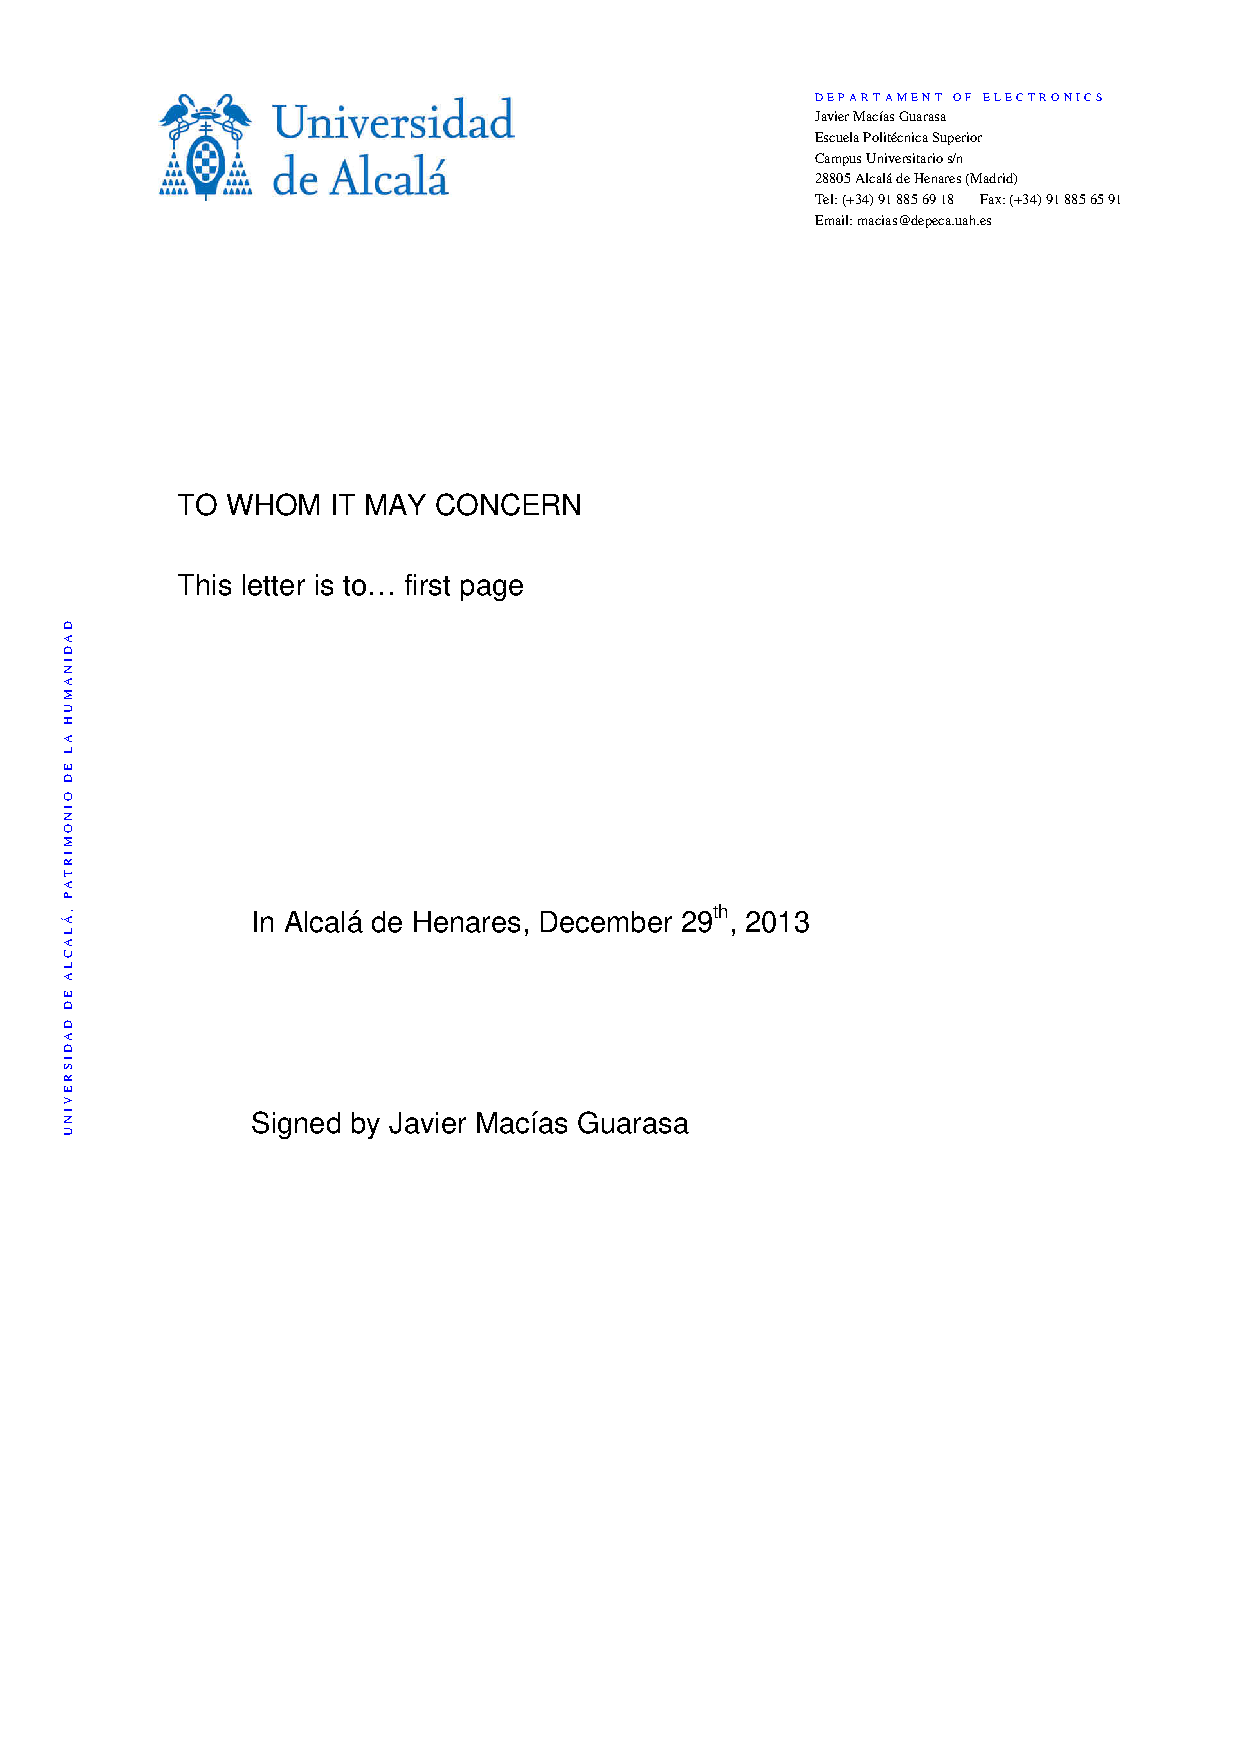
\includepdf[pages=-]{letters/sampleLetter-pages.pdf}   % include all pages of
%                                                 % pdf file
\clearemptydoublepage % You need to add this after including each pdf

%\includepdf[pages=-]{papeleo/vistoBuenoTutorTFM-MUSEA.pdf}   % for TFMs
%\clearemptydoublepage % You need to add this after including each pdf

% Dedication+ackowledgements (dedicatorias+agradecimientos)
%%%%%%%%%%%%%%%%%%%%%%%%%%%%%%%%%%%%%%%%%%%%%%%%%%%%%%%%%%%%%%%%%%%%%%%%%%%
% Función: dedicatoria.
%
% Uso: modifica este fichero para sustituir el ejemplo por tu contenido.
%%%%%%%%%%%%%%%%%%%%%%%%%%%%%%%%%%%%%%%%%%%%%%%%%%%%%%%%%%%%%%%%%%%%%%%%%%%

% 
% This is also courtesy of Roberto Barra
% 
% To center text in a page:
% \topskip0pt
% \vspace*{\fill}
% text
% \vspace*{\fill}

\thispagestyle{empty}

\begin{flushright}

  \topskip0pt
  \vspace*{\fill}

  \textbf{A nuestros alumnos pasados, presentes y futuros\ldots}\\

  \vspace{3cm}

  \emph{``Empieza haciendo lo necesario, luego haz lo posible y de
    pronto empezarás a hacer lo imposible.''}\\ Francisco de Asís

\end{flushright}  

\vspace{4cm}
\vspace*{\fill}

% \clearemptydoublepage



%%% Local Variables:
%%% TeX-master: "../book"
%%% End:
            % EDIT this file or
                                              % comment it out
%%%%%%%%%%%%%%%%%%%%%%%%%%%%%%%%%%%%%%%%%%%%%%%%%%%%%%%%%%%%%%%%%%%%%%%%%%%
% Función: agradecimientos.
%
% Uso: modifica este fichero para sustituir el ejemplo por tu contenido.
%%%%%%%%%%%%%%%%%%%%%%%%%%%%%%%%%%%%%%%%%%%%%%%%%%%%%%%%%%%%%%%%%%%%%%%%%%%

% Use this if you don't like the fancy style
\thispagestyle{empty}

\ifthenelse{\equal{\myLanguage}{english}}
{
  \chapter*{Acknowledgements}
  \label{cha:acknowledgements}
  \markboth{Acknowledgements}{Acknowledgements}
  \addcontentsline{toc}{chapter}{Acknowledgements}
}
{
  \chapter*{Agradecimientos}
  \label{cha:agradecimientos}
  \markboth{Agradecimientos}{Agradecimientos}
  \addcontentsline{toc}{chapter}{Agradecimientos}
}

\begin{FraseCelebre}
  \begin{Frase}
    A todos los que la presente vieren y entendieren.
  \end{Frase}
  \begin{Fuente}
    Inicio de las Leyes Orgánicas. Juan Carlos I
  \end{Fuente}
\end{FraseCelebre}

% ``Más vale un minuto de ilusión que mil horas de
% razonamiento''... (cortesía de Roberto Barra)


Este trabajo es el fruto de muchas horas de trabajo, tanto de los autores últimos de los ficheros de la distribución como de todos los que en mayor o menor medida han participado en él a lo largo de su proceso de gestación.

Mención especial merece Manuel Ocaña, el autor de la primera versión de las plantillas de proyectos fin de carrera y tesis doctorales usadas en el Departamento de Electrónica de la Universidad de Alcalá, con contribuciones de Jesús Nuevo, Pedro Revenga, Fernando Herránz y Noelia Hernández.

En la versión actual, la mayor parte de las definiciones de estilos de partida proceden de la tesis doctoral de Roberto Barra-Chicote, con lo que gracias muy especiales para él.

Añado igualmente a Gonzalo Corral de forma destacada en esta sección por ser el primero que hizo un PR sobre el repositorio github de la plantilla, y que nos llevó del arcaico ISO-8859 de bibtex a la normalidad del UTF-8 de biber (que ya hacía falta).

También damos las gracias a \input{additionalContributors.txt}, que nos han proporcionado secciones completas y/o ejemplos variados de sus tesis o proyectos/trabajos fin de carrera/grado.

Finalmente, hay incontables contribuyentes a esta plantilla, muchos de ellos encontrados gracias a la magia del buscador de Google. Hemos intentado referenciar los más importantes en los fuentes de la plantilla, aunque seguro que hemos omitido alguno. Desde aquí les damos las gracias a todos ellos por compartir su saber y buen hacer con el mundo.

En las últimas revisiones (desde principios de 2025) también cuento con la hechicería de ChatGPT y Codex, dos ayudantes incansables que me han ayudado a reorganizar la documentación, proponer redacciones, localizar incoherencias y revisar los cambios en los fuentes. Las decisiones finales y, por supuesto, los errores que queden, son responsabilidad exclusivamente mía.


% Back to normal JIC. Use it if you set \pagestyle{myplain} above
%\pagestyle{fancy}

%%% Local Variables:
%%% TeX-master: "../book"
%%% End:


  % EDIT this file or
                                              % comment it out

% If this is the case, include definitions of acronyms (it's
% included before resumen.tex and abstract.tex in case you want
% to use them here
%%%%%%%%%%%%%%%%%%%%%%%%%%%%%%%%%%%%%%%%%%%%%%%%%%%%%%%%%%%%%%%%%%%%%%%%%%%
% Función: definición de los acrónimos del documento.
%
% Uso: modifica este fichero para incluir las definiciones de tu trabajo.
%%%%%%%%%%%%%%%%%%%%%%%%%%%%%%%%%%%%%%%%%%%%%%%%%%%%%%%%%%%%%%%%%%%%%%%%%%%

% This file shows some examples for glossary terms

%%%%%%%%%%%%%%%%%%%%%%%%%%%%%%%%%%%%%%%%%%%%%%%%%%%%%%%%%%%%%%%%%%%%%%%%%%%
% BEGIN example of glossary terms definition
%
\newacronym{HMI}{HMI}{Human-Machine Interfaces}
\newacronym{ETTS}{ETTS}{Emotional Text To Speech}
\newacronym{TTS}{TTS}{Text To Speech}
\newacronym{PSOLA}{PSOLA}{Pitch Synchronous OverLap Add}
\newacronym{TDPSOLA}{TD-PSOLA}{Time Domain Pitch Synchronous OverLap Add}
\newacronym{AI}{AI}{Artificial Intelligenge}

\newacronym{SPSS}{SPSS}{Statistical Parametric Speech Synthesis}
\newacronym{VC}{VC}{Voice Conversion}
\newacronym{US}{US}{Unit Selection}
\newacronym{HMM}{HMM}{Hidden Markov Model}
\newacronym{LSP}{LSP}{Line Spectral Pairs}
\newacronym{LPC}{LPC}{Linear Prediction Coefficiens}
\newacronym{LSF}{LSF}{Line Spectral Frequencies}
\newacronym{F0}{F0}{Fundamental Frequency}
\newacronym{MCEP}{MCEP}{Mel Cepstral Coefficients}
\newacronym{MGCEP}{MGCEP}{Mel Generalized Cepstral Coefficients}
\newacronym{MFCC}{MFCC}{Mel Frequency Cepstrum Coefficients}
\newacronym{ASR}{ASR}{Automatic Speech Recognition}
\newacronym{MDL}{MDL}{Minimum Description Length Criterion}
\newacronym{MSD}{MSD}{Multi Space Probability Distributions}
\newacronym{HSMM}{HSMM}{Hidden Semi-Markov Models}
\newacronym{ML}{ML}{Maximum Likelihood}
\newacronym{MLSA}{MLSA}{Mel Log Spectrum Approximation}
\newacronym{MAP}{MAP}{Maximum A Posteriori} 
\newacronym{MLLR}{MLLR}{Maximum Likelihood Linear Regression}
\newacronym{CSMAPLR}{CSMAPLR}{Constrain Structural MAP Linear Regression}
\newacronym{AV}{AV}{Average Voice}

\newacronym{ANN}{ANN}{Artificial Neural Network}

\newacronym{NIST}{NIST}{National Institute of Technology}
\newacronym{SES}{SES}{Spanish Expressive Speech}
\newacronym{EMODB}{EMODB}{Berlin Database of Emotional Speech}

\newacronym{FAUAIBO}{FAU-AIBO}{FAU AIBO Emotion Corpus}

\newacronym{SEV}{SEV}{Spanish Expressive Voices}
\newacronym{AER}{AER}{Automatic Emotion Recognition}
\newacronym{UBEC}{UBEC}{Universal Background Emotion Codebook}

\newacronym{STRAIGHT}{STRAIGHT}{Speech Transformation and Representation using Adaptive Interpolation of weiGHTed spectrum}


\newacronym{DBN}{DBN}{Dynamic Bayesian Network}
\newacronym{SQ}{SQ}{Speech Quality}
\newacronym{EIR}{EIR}{Emotion Identification Rate}
\newacronym{SIR}{SIR}{Speaker Identification Rate}
\newacronym{ES}{ES}{Emotional Strength}

\newacronym{ACCCHARS}{ÁÉÍÓÚÜÑáéíóúüñ}{Long ÁÉÍÓÚÜÑáéíóúüñ}

% In the future version of texlive, we will be able to use longplural
% and shortplural. Right now we must use \newglossaryentry.
%\newacronym[longplural={Systems on a Chip},shortplural={SOCs}]{SOC}{SOC}{System on a Chip}
\newglossaryentry{SOC}{type=\acronymtype,
        name={SOC},
        symbol={},
        sort=soc,
        plural={SOCs},
        firstplural={Systems on a Chip (SOCs)},
        description={System on a Chip},
        descriptionplural={Systems on a Chip}}

%
% END example of glossary terms definition
%%%%%%%%%%%%%%%%%%%%%%%%%%%%%%%%%%%%%%%%%%%%%%%%%%%%%%%%%%%%%%%%%%%%%%%%%%%


%%% Local Variables:
%%% TeX-master: "../book"
%%% End:
            % EDIT this file or
                                              % comment it out if you do
                                              % not use acronyms

% If this is the case, include definitions of acronyms (it's
% included before resumen.tex and abstract.tex in case you want
% to use them there
%%%%%%%%%%%%%%%%%%%%%%%%%%%%%%%%%%%%%%%%%%%%%%%%%%%%%%%%%%%%%%%%%%%%%%%%%%%
% Función: definición de los símbolos del documento.
%
% Uso: modifica este fichero para incluir las definiciones de tu trabajo.
%%%%%%%%%%%%%%%%%%%%%%%%%%%%%%%%%%%%%%%%%%%%%%%%%%%%%%%%%%%%%%%%%%%%%%%%%%%

% These ones for the symbols glossary

%%%%%%%%%%%%%%%%%%%%%%%%%%%%%%%%%%%%%%%%%%%%%%%%%%%%%%%%%%%%%%%%%%%%%%%%%%%
% BEGIN example of symbols definition
%
\newglossaryentry{ohm}{type=symbols,
        name={\ensuremath{\Omega}},
        symbol={\ensuremath{\Omega}}, 
        sort=ohm,
        description=unit of electrical resistance}

\newglossaryentry{angstrom}{type=symbols,
        name={\AA},
        symbol={\AA},
        sort=angstrom,
        description={non-SI unit of length}}

\newglossaryentry{xdet}{type=symbols,
        name={\ensuremath{x(t)}},
        symbol={\ensuremath{x(t)}},
        sort=xdet,
        description={Audio signal}}

\newglossaryentry{xidet}{type=symbols,
        name={\ensuremath{x_i(t)}},
        symbol={\ensuremath{x_i(t)}},
        sort=xidet,
        description={Audio signal captured at microphone $i$}}

\newglossaryentry{condindep}{type=symbols,
        name={\ensuremath{\ci}},
        symbol={\ensuremath{\ci}}, 
        sort=conditionalindependence,
        description=conditional independence}

%
% END example of symbols definition
%%%%%%%%%%%%%%%%%%%%%%%%%%%%%%%%%%%%%%%%%%%%%%%%%%%%%%%%%%%%%%%%%%%%%%%%%%%

%%% Local Variables:
%%% TeX-master: "../book"
%%% End:
              % EDIT this file or
                                              % comment it out if you do
                                              % not use acronyms

% Now include resumen and abstract
%%%%%%%%%%%%%%%%%%%%%%%%%%%%%%%%%%%%%%%%%%%%%%%%%%%%%%%%%%%%%%%%%%%%%%%%%%%
% Función: resumen en español y palabras clave.
%
% Uso: modifica este fichero para sustituir el ejemplo por tu contenido.
%%%%%%%%%%%%%%%%%%%%%%%%%%%%%%%%%%%%%%%%%%%%%%%%%%%%%%%%%%%%%%%%%%%%%%%%%%%

\chapter*{Resumen}
\label{cha:resumen}
\markboth{Resumen}{Resumen}

\addcontentsline{toc}{chapter}{Resumen}

Este documento ha sido generado con una plantilla para memorias de
trabajos fin de carrera, fin de máster, fin de grado y tesis
doctorales. Está especialmente pensado para su uso en la Universidad de
Alcalá, pero debería ser fácilmente extensible y adaptable a otros casos
de uso. En su contenido se incluyen las instrucciones generales para
usarlo, así como algunos ejemplos de elementos que pueden ser de
utilidad. Si tenéis problemas, sugerencias o comentarios sobre el mismo,
dirigidlas por favor a \contactauthor.

\textbf{Palabras clave:} \myThesisKeywords.

%%% Local Variables:
%%% TeX-master: "../book"
%%% End:


                  % EDIT this file
%%%%%%%%%%%%%%%%%%%%%%%%%%%%%%%%%%%%%%%%%%%%%%%%%%%%%%%%%%%%%%%%%%%%%%%%%%%
% Purpose: English abstract and keywords.
%
% Usage: edit this file to replace the sample abstract with your own.
%%%%%%%%%%%%%%%%%%%%%%%%%%%%%%%%%%%%%%%%%%%%%%%%%%%%%%%%%%%%%%%%%%%%%%%%%%%

\chapter*{Abstract}
\label{cha:abstract}

\addcontentsline{toc}{chapter}{Abstract}

This document has been generated with a template for Bsc and Msc Thesis
(trabajos fin de carrera, fin de máster, fin de grado) and PhD. Thesis,
specially thought for its use in Universidad de Alcalá, although it
should be easily extended and adapted for other use cases. In its
content we include general instructions of use, and some example of
elements than can be useful. If you have problemas, suggestions or
comments on the template, please forward them to \contactauthor.


\textbf{Keywords:} \myThesisKeywordsEnglish.

%%% Local Variables:
%%% TeX-master: "../book"
%%% End:


                 % EDIT this file

% Just for TFGs/PFCs at UAH, I do nothing and leave to the author the
% inclusion of the file
%%%%%%%%%%%%%%%%%%%%%%%%%%%%%%%%%%%%%%%%%%%%%%%%%%%%%%%%%%%%%%%%%%%%%%%%%%%%
% Función: resumen extendido.
%
% Uso: modifica este fichero para sustituir el ejemplo por tu contenido.
%%%%%%%%%%%%%%%%%%%%%%%%%%%%%%%%%%%%%%%%%%%%%%%%%%%%%%%%%%%%%%%%%%%%%%%%%%%

\ifthenelse{\equal{\myLanguage}{english}}
{
\chapter*{Extended Abstract}
\label{cha:resumen-extendido}
\markboth{Extended Abstract}{Extended Abstract}

\addcontentsline{toc}{chapter}{Extended Abstract}
}
{
\chapter*{Resumen extendido}
\label{cha:resumen-extendido}
\markboth{Resumen extendido}{Resumen extendido}

\addcontentsline{toc}{chapter}{Resumen extendido}
}

Con un máximo de cuatro o cinco páginas. Se supone que sólo está
definido como obligatorio para los TFGs y PFCs de UAH.

%%% Local Variables:
%%% TeX-master: "../book"
%%% End:


       % EDIT this file

% Now include toc and list of figures+tables
%%%%%%%%%%%%%%%%%%%%%%%%%%%%%%%%%%%%%%%%%%%%%%%%%%%%%%%%%%%%%%%%%%%%%%%%%%%
%
% Generic template for TFC/TFM/TFG/Tesis
%
% $Id: toc+lof+lot.tex,v 1.9 2015/06/05 00:10:34 macias Exp $
%
% By:
%  + Javier Macías-Guarasa. 
%    Departamento de Electrónica
%    Universidad de Alcalá
%  + Roberto Barra-Chicote. 
%    Departamento de Ingeniería Electrónica
%    Universidad Politécnica de Madrid   
% 
% Based on original sources by Roberto Barra, Manuel Ocaña, Jesús Nuevo,
% Pedro Revenga, Fernando Herránz and Noelia Hernández. Thanks a lot to
% all of them, and to the many anonymous contributors found (thanks to
% google) that provided help in setting all this up.
%
% See also the additionalContributors.txt file to check the name of
% additional contributors to this work.
%
% If you think you can add pieces of relevant/useful examples,
% improvements, please contact us at (macias@depeca.uah.es)
%
% You can freely use this template and please contribute with
% comments or suggestions!!!
%
%%%%%%%%%%%%%%%%%%%%%%%%%%%%%%%%%%%%%%%%%%%%%%%%%%%%%%%%%%%%%%%%%%%%%%%%%%%

\clearemptydoublepage
\hypersetup{linkcolor=\mytoclinkcolor}
\tableofcontents

\ifthenelse{\equal{\myIncludeListOfFigures}{true}}
{
  \clearemptydoublepage
  \hypersetup{linkcolor=\myloflinkcolor}
  \listoffigures
}
{}

\ifthenelse{\equal{\myIncludeListOfTables}{true}}
{
  \clearemptydoublepage
  \hypersetup{linkcolor=\mylotlinkcolor}
  \listoftables
}
{}

\hypersetup{linkcolor=\mylinkcolor}

%%% Local Variables:
%%% TeX-master: "../book"
%%% End:
                 % DO NOT TOUCH THIS LINE!

% If you want to include additional listings, you can use the float
% package. As an example, I include here the listing of source code
% snippets and algorithms (you have some examples in
% appendix/codigo-algoritmos-listados.tex)
%%%%%%%%%%%%%%%%%%%%%%%%%%%%%%%%%%%%%%%%%%%%%%%%%%%%%%%%%%%%%%%%%%%%%%%%%%%
%
% Generic template for TFC/TFM/TFG/Tesis
%
% $Id: extralistings.tex,v 1.5 2015/06/05 00:10:34 macias Exp $
%
% By:
%  + Javier Macías-Guarasa. 
%    Departamento de Electrónica
%    Universidad de Alcalá
%  + Roberto Barra-Chicote. 
%    Departamento de Ingeniería Electrónica
%    Universidad Politécnica de Madrid   
% 
% Based on original sources by Roberto Barra, Manuel Ocaña, Jesús Nuevo,
% Pedro Revenga, Fernando Herránz and Noelia Hernández. Thanks a lot to
% all of them, and to the many anonymous contributors found (thanks to
% google) that provided help in setting all this up.
%
% See also the additionalContributors.txt file to check the name of
% additional contributors to this work.
%
% If you think you can add pieces of relevant/useful examples,
% improvements, please contact us at (macias@depeca.uah.es)
%
% You can freely use this template and please contribute with
% comments or suggestions!!!
%
%%%%%%%%%%%%%%%%%%%%%%%%%%%%%%%%%%%%%%%%%%%%%%%%%%%%%%%%%%%%%%%%%%%%%%%%%%%

% Include the list of source code listings (if this is the case)
\hypersetup{linkcolor=\myothertoclinkcolor}
\ifthenelse{\equal{\myIncludeListOfCode}{true}}
{
  \ifthenelse{\equal{\myLanguage}{english}}
  {
    \listof{codefloat}{List of source code listings}
    \addcontentsline{toc}{chapter}{List of source code listings}
  }
  {
    \listof{codefloat}{Índice de listados de código fuente}
    \addcontentsline{toc}{chapter}{Índice de listados de código fuente}
  }
}
{}

\ifthenelse{\equal{\myIncludeListOfAlgorithms}{true}}
{
  \ifthenelse{\equal{\myLanguage}{english}}
  {
    \renewcommand*{\algorithmcfname}{Algorithm}
    \renewcommand{\listofalgorithms}{\begingroup
      \tocfile{List of Algorithms}{loa}
      \endgroup}
  }
  {
    \renewcommand*{\algorithmcfname}{Algoritmo}
    \renewcommand{\listofalgorithms}{\begingroup
      \tocfile{Índice de algoritmos}{loa}
      \endgroup}
  }
  \listofalgorithms
  \clearemptydoublepage
}
{}

\hypersetup{linkcolor=\myothertoclinkcolor}
% This is code to add a list of videos if used
\ifthenelse{\equal{\myIncludeListOfVideos}{true}}
{
  \ifthenelse{\equal{\myLanguage}{english}}
  {
    \listofvideos
    \addcontentsline{toc}{chapter}{List of videos}
  }
  {
    \listofvideos
    \addcontentsline{toc}{chapter}{Índice de vídeos}
  }
}
{}

\hypersetup{linkcolor=\mylinkcolor}


%%% Local Variables:
%%% TeX-master: "../book"
%%% End:
               % Edit this file or
                                              % comment it out

% Now include list of acronyms and options (if this is the case)
%%%%%%%%%%%%%%%%%%%%%%%%%%%%%%%%%%%%%%%%%%%%%%%%%%%%%%%%%%%%%%%%%%%%%%%%%%%
% Función: listado de acrónimos.
%
% Uso: inclusión automática; normalmente no debes modificarlo.
% No se compila por separado.
%%%%%%%%%%%%%%%%%%%%%%%%%%%%%%%%%%%%%%%%%%%%%%%%%%%%%%%%%%%%%%%%%%%%%%%%%%%

% You can change the way the entries appear the first time they are
% used. I've used italics by default. I found a problem if using this:
% LaTeX adds an extra space after the acronym, so I'm commenting it out
% (if you find a solution, please let me know)
%\defglsdisplayfirst[\acronymtype]{\textit{#1}} % EDIT this if required

% This may lead to problems... I don't know how to fix it in case the
% column for acronym is wider than 0.3\linewidth
\setlength{\glsdescwidth}{0.7\linewidth}       % EDIT this if required

% Set language specific definitions...
\begin{thesislisttitlestyle}
\ifthenelse{\equal{\myLanguage}{english}}
{
\printglossary[type=\acronymtype,style=long,nonumberlist=true,title=List of Acronyms,toctitle=List of Acronyms]
\addcontentsline{toc}{chapter}{List of Acronyms}
}
{
\printglossary[type=\acronymtype,style=long,nonumberlist=true,title=Lista de acrónimos,toctitle=Lista de acrónimos]
\addcontentsline{toc}{chapter}{Lista de acrónimos}
}
\end{thesislisttitlestyle}


%%% Local Variables:
%%% TeX-master: "../book"
%%% End:

               % EDIT this file or
                                              % comment it out if you do
                                              % not use acronyms

% Now include symbols of symbols and options (if this is the case)
%%%%%%%%%%%%%%%%%%%%%%%%%%%%%%%%%%%%%%%%%%%%%%%%%%%%%%%%%%%%%%%%%%%%%%%%%%%
% Función: listado de símbolos.
%
% Uso: inclusión automática; normalmente no debes modificarlo.
% No se compila por separado.
%%%%%%%%%%%%%%%%%%%%%%%%%%%%%%%%%%%%%%%%%%%%%%%%%%%%%%%%%%%%%%%%%%%%%%%%%%%

% Set language specific definitions...
\begin{thesislisttitlestyle}
\ifthenelse{\equal{\myLanguage}{english}}
{
  \printglossary[type=symbols,style=long,nonumberlist=true,title=List of Symbols,toctitle=List of Symbols]
  \addcontentsline{toc}{chapter}{List of Symbols}
}
{
  \printglossary[type=symbols,style=long,nonumberlist=true,title=Lista de símbolos,title=Lista de símbolos,toctitle=Lista de símbolos]
  \addcontentsline{toc}{chapter}{Lista de símbolos}
}
\end{thesislisttitlestyle}


%%% Local Variables:
%%% TeX-master: "../book"
%%% End:
                 % EDIT this file or
                                              % comment it out if you do
                                              % not use acronyms

%
% END within-document configuration, frontpage and cover pages generation
%%%%%%%%%%%%%%%%%%%%%%%%%%%%%%%%%%%%%%%%%%%%%%%%%%%%%%%%%%%%%%%%%%%%%%%%%%%

%%%%%%%%%%%%%%%%%%%%%%%%%%%%%%%%%%%%%%%%%%%%%%%%%%%%%%%%%%%%%%%%%%%%%%%%%%%
% Now start text and numbering for mainmatter (chapter+appendices)
%%%%%%%%%%%%%%%%%%%%%%%%%%%%%%%%%%%%%%%%%%%%%%%%%%%%%%%%%%%%%%%%%%%%%%%%%%%
\mainmatter                                       % DO NOT TOUCH THIS LINE!

\ifthenelse{\equal{\myLanguage}{english}}         % DO NOT TOUCH THIS LINE!
  {\part{Extended Summary of the Thesis}}         % DO NOT TOUCH THIS LINE!
  {\part{Resumen extendido de la tesis}}          % DO NOT TOUCH THIS LINE!
\label{part:compendium-summary}                   % DO NOT TOUCH THIS LINE!

%%%%%%%%%%%%%%%%%%%%%%%%%%%%%%%%%%%%%%%%%%%%%%%%%%%%%%%%%%%%%%%%%%%%%%%%%%%
%%%%%%%%%%%%%%%%%%%%%%%%%%%%%%%%%%%%%%%%%%%%%%%%%%%%%%%%%%%%%%%%%%%%%%%%%%%
%%%%%%%%%%%%%%%%%%%%%%%%%%%%%%%%%%%%%%%%%%%%%%%%%%%%%%%%%%%%%%%%%%%%%%%%%%%
%%%%%%%%%%%%%%%%%%%%%%%%%%%%%%%%%%%%%%%%%%%%%%%%%%%%%%%%%%%%%%%%%%%%%%%%%%%
%%%%%%%%%%%%%%%%%%%%%%%%%%%%%%%%%%%%%%%%%%%%%%%%%%%%%%%%%%%%%%%%%%%%%%%%%%%
%%%%%%%%%%%%%%%%%%%%%%%%%%%%%%%%%%%%%%%%%%%%%%%%%%%%%%%%%%%%%%%%%%%%%%%%%%%
%%%%%%%%%%%%%%%%%%%%%%%%%%%%%%%%%%%%%%%%%%%%%%%%%%%%%%%%%%%%%%%%%%%%%%%%%%%
% BEGIN Normal chapters for the Thesis Summary. Edit/modify all within this section

% Part I: synthetic account of the complete thesis.
%%%%%%%%%%%%%%%%%%%%%%%%%%%%%%%%%%%%%%%%%%%%%%%%%%%%%%%%%%%%%%%%%%%%%%%%%%%
% Función: capítulo de ejemplo de introducción de la tesis por compendio.
%
% Uso: modifica este fichero para adaptar el contenido a tu trabajo.
%%%%%%%%%%%%%%%%%%%%%%%%%%%%%%%%%%%%%%%%%%%%%%%%%%%%%%%%%%%%%%%%%%%%%%%%%%%

\ifthenelse{\equal{\myLanguage}{english}}
{
  \chapter{Introduction}
}
{
  \chapter{Introducción}
}
\label{cha:compendium-introduction}

\ifthenelse{\equal{\myLanguage}{english}}
{
  \section{Context and Motivation}
  \subsection{Research context}
}
{
  \section{Contexto y motivación}
  \subsection{Contexto de la investigación}
}

\ifthenelse{\equal{\myLanguage}{english}}
{
  Use this chapter to introduce the research context, motivation and central problem addressed by the thesis. Explain why the problem is relevant, delimit the scope of the work and provide the reader with the information required to understand the extended summary. This sample also demonstrates the use of acronyms: \gls{AI} and \gls{HMI}.
}
{
  Utiliza este capítulo para presentar el contexto de la investigación, su motivación y el problema central abordado por la tesis. Explica por qué el problema es relevante, delimita el alcance del trabajo y proporciona la información necesaria para comprender el resumen extendido. Este ejemplo también muestra el uso de acrónimos: \gls{AI} y \gls{HMI}.
}

\ifthenelse{\equal{\myLanguage}{english}}
{
  \subsection{Problem statement}

  Define the specific problem addressed by the thesis, its scope and the assumptions that delimit the proposed research.

  \section{Organization of the Thesis}

  Briefly describe the contents of the extended summary and explain how the publications included in Part~\ref{part:compendium-publications} support the thesis narrative.
}
{
  \subsection{Planteamiento del problema}

  Define el problema concreto abordado por la tesis, su alcance y las hipótesis que delimitan la investigación propuesta.

  \section{Organización de la tesis}

  Describe brevemente el contenido del resumen extendido y explica cómo las publicaciones incluidas en la parte~\ref{part:compendium-publications} sustentan el hilo argumental de la tesis.
}

%%% Local Variables:
%%% TeX-master: "../../book"
%%% End:

\ifthenelse{\equal{\myLanguage}{english}}
{
  \chapter{Objectives}
}
{
  \chapter{Objetivos}
}
\label{cha:compendium-objectives}

\ifthenelse{\equal{\myLanguage}{english}}
{
  \section{General Objective}
}
{
  \section{Objetivo general}
}

\ifthenelse{\equal{\myLanguage}{english}}
{
  State the main hypothesis or general objective of the thesis and derive the specific objectives addressed by the publications. Make the relationship between these objectives and the organization of the extended summary explicit.
}
{
  Expón la hipótesis principal o el objetivo general de la tesis y deriva los objetivos específicos abordados por las publicaciones. Haz explícita la relación entre estos objetivos y la organización del resumen extendido.
}

\ifthenelse{\equal{\myLanguage}{english}}
{
  \section{Specific Objectives}
  \subsection{Scientific objectives}

  Identify the knowledge advances pursued by the thesis and relate each one to the research questions.

  \subsection{Technical and validation objectives}

  Describe the implementation, experimentation and validation goals that make the scientific objectives measurable.
}
{
  \section{Objetivos específicos}
  \subsection{Objetivos científicos}

  Identifica los avances de conocimiento perseguidos por la tesis y relaciona cada uno con las preguntas de investigación.

  \subsection{Objetivos técnicos y de validación}

  Describe los objetivos de implementación, experimentación y validación que permiten evaluar los objetivos científicos.
}

%%% Local Variables:
%%% TeX-master: "../../book"
%%% End:

%%%%%%%%%%%%%%%%%%%%%%%%%%%%%%%%%%%%%%%%%%%%%%%%%%%%%%%%%%%%%%%%%%%%%%%%%%%
% Función: capítulo de ejemplo de trabajos previos de la tesis por compendio.
%
% Uso: modifica este fichero para adaptar el contenido a tu trabajo.
%%%%%%%%%%%%%%%%%%%%%%%%%%%%%%%%%%%%%%%%%%%%%%%%%%%%%%%%%%%%%%%%%%%%%%%%%%%

\ifthenelse{\equal{\myLanguage}{english}}
{
  \chapter{Previous Work}
}
{
  \chapter{Trabajo previo}
}
\label{cha:compendium-previous-work}

\ifthenelse{\equal{\myLanguage}{english}}
{
  \section{Scientific Background}
  \subsection{Foundational approaches}
}
{
  \section{Antecedentes científicos}
  \subsection{Enfoques fundamentales}
}

\ifthenelse{\equal{\myLanguage}{english}}
{
  Review the scientific and technical background of the thesis here. Organize the discussion around the research questions rather than presenting an isolated list of publications, and identify the limitations that motivate the doctoral work.
}
{
  Revisa aquí los antecedentes científicos y técnicos de la tesis. Organiza la discusión alrededor de las preguntas de investigación en lugar de presentar una lista aislada de publicaciones, e identifica las limitaciones que motivan el trabajo doctoral.
}

\ifthenelse{\equal{\myLanguage}{english}}
{
  \subsection{Recent developments}

  Summarize the approaches most directly related to the thesis and compare their assumptions, strengths and limitations.

  \section{Research Gap}

  Conclude the review by identifying the unresolved questions addressed by the objectives of this thesis.
}
{
  \subsection{Desarrollos recientes}

  Resume los enfoques más relacionados con la tesis y compara sus hipótesis, fortalezas y limitaciones.

  \section{Oportunidad de investigación}

  Concluye la revisión identificando las cuestiones no resueltas que abordan los objetivos de esta tesis.
}

%%% Local Variables:
%%% TeX-master: "../../book"
%%% End:

%%%%%%%%%%%%%%%%%%%%%%%%%%%%%%%%%%%%%%%%%%%%%%%%%%%%%%%%%%%%%%%%%%%%%%%%%%%
% Función: capítulo de ejemplo de metodología de la tesis por compendio.
%
% Uso: modifica este fichero para adaptar el contenido a tu trabajo.
%%%%%%%%%%%%%%%%%%%%%%%%%%%%%%%%%%%%%%%%%%%%%%%%%%%%%%%%%%%%%%%%%%%%%%%%%%%

\ifthenelse{\equal{\myLanguage}{english}}
{
  \chapter{Methodology}
}
{
  \chapter{Metodología}
}
\label{cha:compendium-methodology}

\ifthenelse{\equal{\myLanguage}{english}}
{
  \section{Research Design}
  \subsection{General approach}
}
{
  \section{Diseño de la investigación}
  \subsection{Enfoque general}
}

\ifthenelse{\equal{\myLanguage}{english}}
{
  Describe the common methodology connecting the publications, including the experimental design, data, analytical procedures and validation criteria. Refer to the included publications for details while keeping this chapter understandable as a coherent account of the thesis methodology.
}
{
  Describe la metodología común que conecta las publicaciones, incluidos el diseño experimental, los datos, los procedimientos de análisis y los criterios de validación. Remite a las publicaciones incluidas para los detalles, manteniendo este capítulo como una explicación coherente de la metodología de la tesis.
}

\ifthenelse{\equal{\myLanguage}{english}}
{
  \subsection{Data and experimental protocol}

  Explain how the data are obtained, prepared and divided, and identify the variables and controls used throughout the publications.

  \section{Evaluation Methodology}
}
{
  \subsection{Datos y protocolo experimental}

  Explica cómo se obtienen, preparan y dividen los datos, e identifica las variables y los controles utilizados en el conjunto de las publicaciones.

  \section{Metodología de evaluación}
}

\ifthenelse{\equal{\myLanguage}{english}}
{
  Figure~\ref{fig:compendium-example} and Table~\ref{tab:compendium-example} are simple examples that you can replace with material from your thesis.
}
{
  La figura~\ref{fig:compendium-example} y la tabla~\ref{tab:compendium-example} son ejemplos sencillos que puedes sustituir por material de tu tesis.
}

\begin{figure}[htbp]
  \centering
  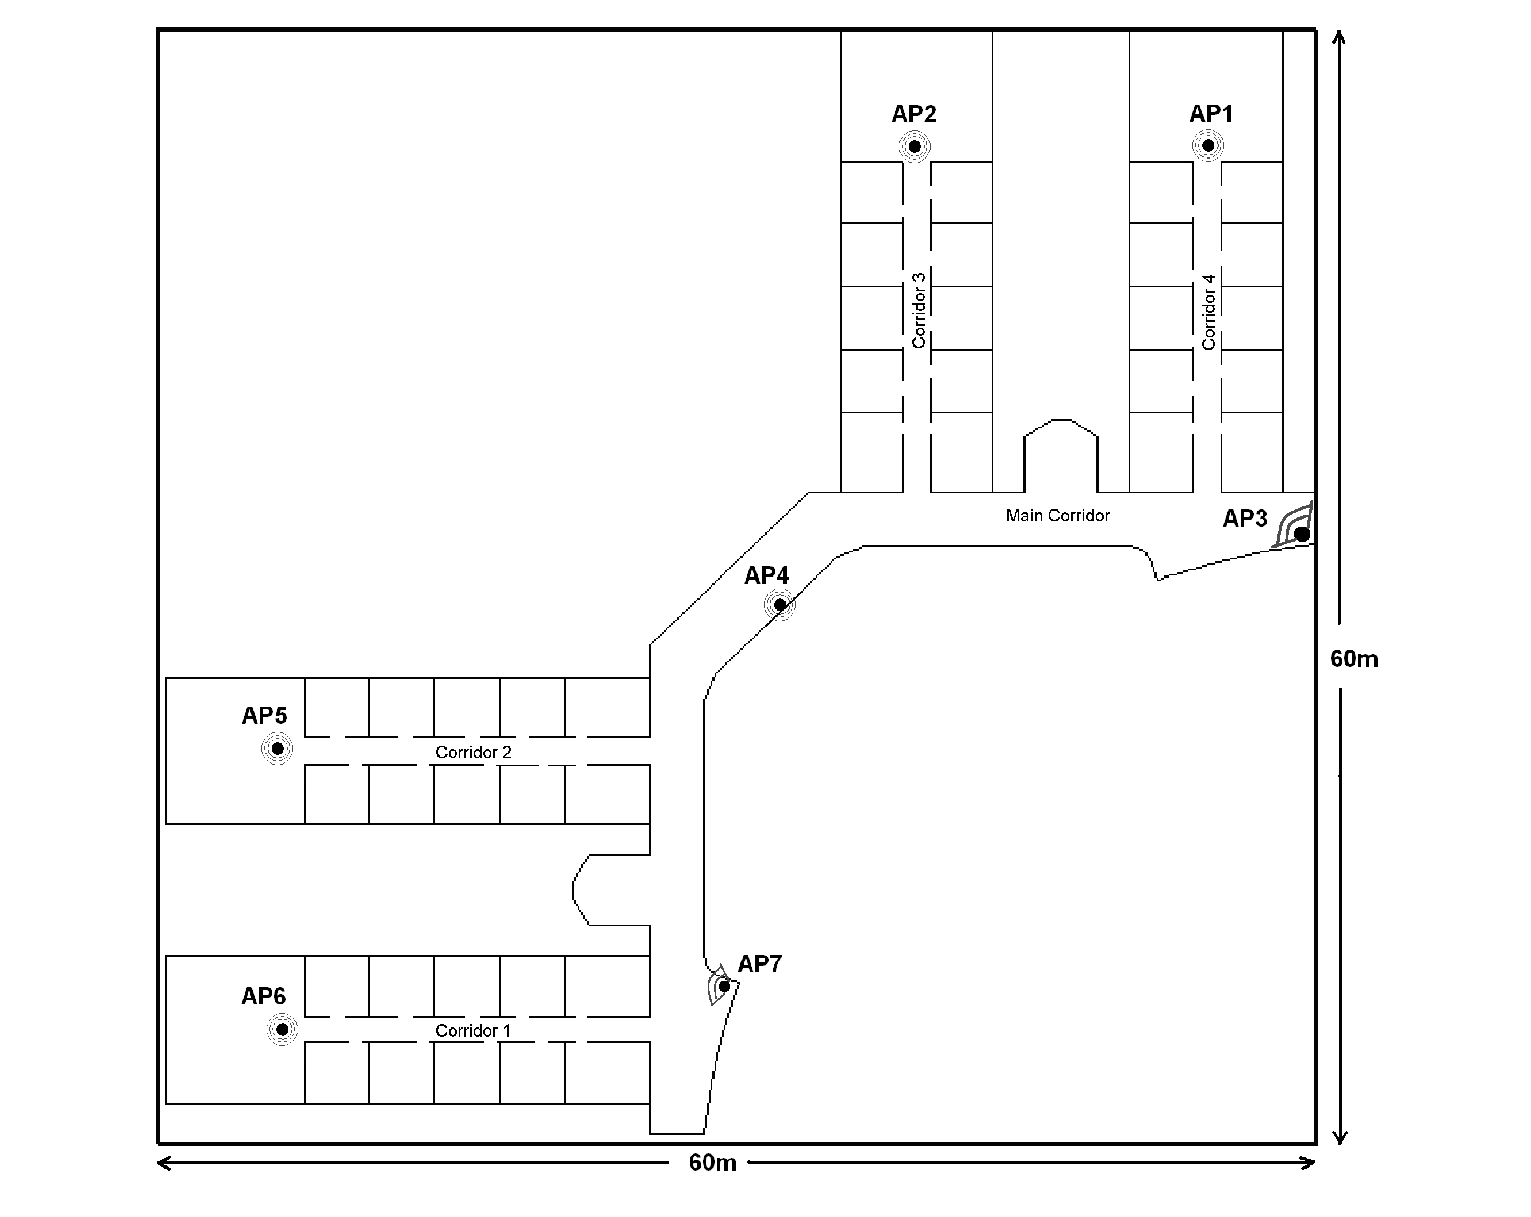
\includegraphics[width=0.55\textwidth]{Figure1}
  \ifthenelse{\equal{\myLanguage}{english}}
  {
    \caption{Example figure in the extended summary.}
  }
  {
    \caption{Ejemplo de figura en el resumen extendido.}
  }
  \label{fig:compendium-example}
\end{figure}

\begin{table}[htbp]
  \centering
  \renewcommand{\arraystretch}{1.2}
  \ifthenelse{\equal{\myLanguage}{english}}
  {
    \caption{Example comparison of experimental results.}
  }
  {
    \caption{Ejemplo de comparación de resultados experimentales.}
  }
  \label{tab:compendium-example}
  \begin{tabular}{|l|c|c|}
    \hline
    \ifthenelse{\equal{\myLanguage}{english}}{Method}{Método} &
    \ifthenelse{\equal{\myLanguage}{english}}{Metric A}{Métrica A} &
    \ifthenelse{\equal{\myLanguage}{english}}{Metric B}{Métrica B} \\
    \hline
    \ifthenelse{\equal{\myLanguage}{english}}{Baseline}{Referencia} & 0.72 & 0.68 \\
    \hline
    \ifthenelse{\equal{\myLanguage}{english}}{Proposed method}{Método propuesto} & 0.84 & 0.79 \\
    \hline
  \end{tabular}
\end{table}

%%% Local Variables:
%%% TeX-master: "../../book"
%%% End:

%%%%%%%%%%%%%%%%%%%%%%%%%%%%%%%%%%%%%%%%%%%%%%%%%%%%%%%%%%%%%%%%%%%%%%%%%%%
% Función: capítulo de ejemplo de contribuciones de la tesis de la tesis por compendio.
%
% Uso: modifica este fichero para adaptar el contenido a tu trabajo.
%%%%%%%%%%%%%%%%%%%%%%%%%%%%%%%%%%%%%%%%%%%%%%%%%%%%%%%%%%%%%%%%%%%%%%%%%%%

\ifthenelse{\equal{\myLanguage}{english}}
{
  \chapter{Thesis Contributions}
}
{
  \chapter{Contribuciones de la tesis}
}
\label{cha:compendium-contributions}

\ifthenelse{\equal{\myLanguage}{english}}
{
  \section{Overview of the Contributions}

  Present and discuss the original contributions of the thesis. Explain how the publications relate to one another, which objective each publication addresses and how their combined results constitute a unified doctoral contribution. The three fictional papers distributed with this example illustrate how to cite each included publication while discussing its contribution~\cite{garcia2026paper1,garcia2026paper2,garcia2026paper3}.

  \subsection{Relationship between the publications}

  Explain the role of each publication and the progression from the initial research question to the combined results of the thesis.

  \section{Supporting Research Material}
  \subsection{Videos and demonstrations}

  Remember that you can very easily include links to videos in the document, and that a list similar to the lists of tables, figures, or algorithms will be generated automatically. The command is defined in \texttt{Config/postamble.tex}, while the list is rendered from \texttt{cover/list-of-videos.tex}. To use it, simply include elements such as \videoLink{Feedback amplifiers: motivation}{https://youtu.be/9xXuasS8B3M} or \videoLink{Feedback amplifiers: ideal theory}{https://youtu.be/ZGMwGX7VCbg}.

  \subsection{Algorithms and source code}

  You can also include algorithms such as Algorithm~\ref{alg:restriction}, and symbols such as~\ac{xidet}.

  In addition, you can include source code listings such as the one shown in Listing~\ref{cod:sample2}.
}
{
  \section{Resumen de las contribuciones}

  Presenta y discute las contribuciones originales de la tesis. Explica cómo se relacionan las publicaciones entre sí, qué objetivo aborda cada una y cómo sus resultados combinados constituyen una contribución doctoral unificada. Los tres artículos ficticios distribuidos con este ejemplo muestran cómo citar cada publicación incluida al discutir su contribución~\cite{garcia2026paper1,garcia2026paper2,garcia2026paper3}.

  \subsection{Relación entre las publicaciones}

  Explica el papel de cada publicación y la progresión desde la pregunta inicial de investigación hasta los resultados conjuntos de la tesis.

  \section{Material de apoyo a la investigación}
  \subsection{Vídeos y demostraciones}

  Recuerda que puedes incluir muy fácilmente enlaces a vídeos en el documento y generar automáticamente un listado similar al de tablas, figuras o algoritmos. La orden se define en \texttt{Config/postamble.tex}, mientras que el listado se genera desde \texttt{cover/list-of-videos.tex}. Para usarla, basta con que incluyas elementos similares a \videoLink{Amplificadores realimentados: motivación}{https://youtu.be/9xXuasS8B3M} o \videoLink{Amplificadores realimentados: teoría ideal}{https://youtu.be/ZGMwGX7VCbg}.

  \subsection{Algoritmos y código fuente}

  Y también puedes incluir algoritmos como el algoritmo~\ref{alg:restriction}, y símbolos como~\ac{xidet}.

  Además de listados de código fuente como en el listado~\ref{cod:sample2}.

}

\begin{algorithm}
  \caption{IntervalRestriction\label{IR}}
  \label{alg:restriction}
  \DontPrintSemicolon
  % \dontprintsemicolon
  \KwData{$G=(X,U)$ such that $G^{tc}$ is an order.}
  \KwResult{$G'=(X,V)$ with $V\subseteq U$ such that $G'^{tc}$ is an
    interval order.}
  \Begin{
    $V \longleftarrow U$\;
    $S \longleftarrow \emptyset$\;
    \For{$x\in X$}{
      $NbSuccInS(x) \longleftarrow 0$\;
      $NbPredInMin(x) \longleftarrow 0$\;
      $NbPredNotInMin(x) \longleftarrow |ImPred(x)|$\;
    }
    \For{$x \in X$}{
      \If{$NbPredInMin(x) = 0$ {\bf and} $NbPredNotInMin(x) = 0$}{
        $AppendToMin(x)$}
    }
    \nl\While{$S \neq \emptyset$}{\label{InRes1}
      \nlset{REM} remove $x$ from the list of $T$ of maximal index\;\label{InResR}
      \lnl{InRes2}\While{$|S \cap ImSucc(x)| \neq |S|$}{
        \For{$ y \in S-ImSucc(x)$}{
          \{ remove from $V$ all the arcs $zy$ : \}\;
          \For{$z \in ImPred(y) \cap Min$}{
            remove the arc $zy$ from $V$\;
            $NbSuccInS(z) \longleftarrow NbSuccInS(z) - 1$\;
            move $z$ in $T$ to the list preceding its present list\;
            \{i.e. If $z \in T[k]$, move $z$ from $T[k]$ to
            $T[k-1]$\}\;
          }
          $NbPredInMin(y) \longleftarrow 0$\;
          $NbPredNotInMin(y) \longleftarrow 0$\;
          $S \longleftarrow S - \{y\}$\;
          $AppendToMin(y)$\;
        }
      }
      $RemoveFromMin(x)$\;
    }
  }
\end{algorithm}


\begin{codefloat}
\lstinputlisting[style=Cnice]{appendix/hello.c}
\caption{Ejemplo de código fuente con estilo \texttt{Cnice}, de nuevo
  con un \texttt{lstinputlisting} dentro de un \texttt{codefloat}}
\label{cod:sample2}
\end{codefloat}

%%% Local Variables:
%%% TeX-master: "../../book"
%%% End:

\ifthenelse{\equal{\myLanguage}{english}}
{
  \chapter{Conclusions and Future Work}
}
{
  \chapter{Conclusiones y líneas futuras}
}
\label{cha:compendium-conclusions}

\ifthenelse{\equal{\myLanguage}{english}}
{
  \section{Main Conclusions}
}
{
  \section{Conclusiones principales}
}

\ifthenelse{\equal{\myLanguage}{english}}
{
  Summarize the conclusions supported by the thesis as a whole, relate them to the objectives and discuss the principal limitations. Close the extended summary by identifying research directions that follow from the results.
}
{
  Resume las conclusiones sustentadas por el conjunto de la tesis, relaciónalas con los objetivos y discute las principales limitaciones. Cierra el resumen extendido identificando las líneas de investigación que se derivan de los resultados.
}

\ifthenelse{\equal{\myLanguage}{english}}
{
  \section{Limitations}

  Discuss the assumptions and practical constraints that limit the generalization of the results and should be considered when interpreting the conclusions.

  \section{Future Research Directions}
  \subsection{Immediate extensions}

  Identify improvements and experiments that follow directly from the work presented in the thesis.

  \subsection{Long-term research opportunities}

  Outline broader questions opened by the combined contributions and publications.
}
{
  \section{Limitaciones}

  Discute las hipótesis y restricciones prácticas que limitan la generalización de los resultados y deben considerarse al interpretar las conclusiones.

  \section{Líneas futuras de investigación}
  \subsection{Extensiones inmediatas}

  Identifica las mejoras y experimentos que se derivan directamente del trabajo presentado en la tesis.

  \subsection{Oportunidades de investigación a largo plazo}

  Plantea cuestiones más amplias abiertas por el conjunto de las contribuciones y publicaciones.
}

%%% Local Variables:
%%% TeX-master: "../../book"
%%% End:



%
% END Normal chapters. Edit/modify all within this section
%%%%%%%%%%%%%%%%%%%%%%%%%%%%%%%%%%%%%%%%%%%%%%%%%%%%%%%%%%%%%%%%%%%%%%%%%%%
%%%%%%%%%%%%%%%%%%%%%%%%%%%%%%%%%%%%%%%%%%%%%%%%%%%%%%%%%%%%%%%%%%%%%%%%%%%
%%%%%%%%%%%%%%%%%%%%%%%%%%%%%%%%%%%%%%%%%%%%%%%%%%%%%%%%%%%%%%%%%%%%%%%%%%%
%%%%%%%%%%%%%%%%%%%%%%%%%%%%%%%%%%%%%%%%%%%%%%%%%%%%%%%%%%%%%%%%%%%%%%%%%%%
%%%%%%%%%%%%%%%%%%%%%%%%%%%%%%%%%%%%%%%%%%%%%%%%%%%%%%%%%%%%%%%%%%%%%%%%%%%
%%%%%%%%%%%%%%%%%%%%%%%%%%%%%%%%%%%%%%%%%%%%%%%%%%%%%%%%%%%%%%%%%%%%%%%%%%%
%%%%%%%%%%%%%%%%%%%%%%%%%%%%%%%%%%%%%%%%%%%%%%%%%%%%%%%%%%%%%%%%%%%%%%%%%%%


%%%%%%%%%%%%%%%%%%%%%%%%%%%%%%%%%%%%%%%%%%%%%%%%%%%%%%%%%%%%%%%%%%%%%%%%%%%
% Bibliography for the extended summary. Bibliography processing remains
% configured through BibLaTeX and Biber in the shared Config files.
%%%%%%%%%%%%%%%%%%%%%%%%%%%%%%%%%%%%%%%%%%%%%%%%%%%%%%%%%%%%%%%%%%%%%%%%%%%
%%%%%%%%%%%%%%%%%%%%%%%%%%%%%%%%%%%%%%%%%%%%%%%%%%%%%%%%%%%%%%%%%%%%%%%%%%%
% Función: bibliografía.
%
% Uso: inclusión automática; normalmente no debes modificarlo.
% No se compila por separado.
%%%%%%%%%%%%%%%%%%%%%%%%%%%%%%%%%%%%%%%%%%%%%%%%%%%%%%%%%%%%%%%%%%%%%%%%%%%

% IMPORTANT: YOU DON'T HAVE TO EDIT THIS FILE, JUST EDIT THE bibliofiles.tex file
% IMPORTANT: YOU DON'T HAVE TO EDIT THIS FILE, JUST EDIT THE bibliofiles.tex file
% IMPORTANT: YOU DON'T HAVE TO EDIT THIS FILE, JUST EDIT THE bibliofiles.tex file
% IMPORTANT: YOU DON'T HAVE TO EDIT THIS FILE, JUST EDIT THE bibliofiles.tex file
% IMPORTANT: YOU DON'T HAVE TO EDIT THIS FILE, JUST EDIT THE bibliofiles.tex file
% IMPORTANT: YOU DON'T HAVE TO EDIT THIS FILE, JUST EDIT THE bibliofiles.tex file
% IMPORTANT: YOU DON'T HAVE TO EDIT THIS FILE, JUST EDIT THE bibliofiles.tex file
% IMPORTANT: YOU DON'T HAVE TO EDIT THIS FILE, JUST EDIT THE bibliofiles.tex file
% IMPORTANT: YOU DON'T HAVE TO EDIT THIS FILE, JUST EDIT THE bibliofiles.tex file
% IMPORTANT: YOU DON'T HAVE TO EDIT THIS FILE, JUST EDIT THE bibliofiles.tex file
% IMPORTANT: YOU DON'T HAVE TO EDIT THIS FILE, JUST EDIT THE bibliofiles.tex file
% IMPORTANT: YOU DON'T HAVE TO EDIT THIS FILE, JUST EDIT THE bibliofiles.tex file
% IMPORTANT: YOU DON'T HAVE TO EDIT THIS FILE, JUST EDIT THE bibliofiles.tex file
% IMPORTANT: YOU DON'T HAVE TO EDIT THIS FILE, JUST EDIT THE bibliofiles.tex file
% IMPORTANT: YOU DON'T HAVE TO EDIT THIS FILE, JUST EDIT THE bibliofiles.tex file
% IMPORTANT: YOU DON'T HAVE TO EDIT THIS FILE, JUST EDIT THE bibliofiles.tex file
% IMPORTANT: YOU DON'T HAVE TO EDIT THIS FILE, JUST EDIT THE bibliofiles.tex file
% IMPORTANT: YOU DON'T HAVE TO EDIT THIS FILE, JUST EDIT THE bibliofiles.tex file
% IMPORTANT: YOU DON'T HAVE TO EDIT THIS FILE, JUST EDIT THE bibliofiles.tex file
% IMPORTANT: YOU DON'T HAVE TO EDIT THIS FILE, JUST EDIT THE bibliofiles.tex file
% IMPORTANT: YOU DON'T HAVE TO EDIT THIS FILE, JUST EDIT THE bibliofiles.tex file


\ifthenelse{\equal{\bibliosystem}{biblatex}}
{
  % Use biblatex instead of bibtex

  %% Wen changing to biblatex, we could not define here the bibliography files, so that
  %% You need to edit the bibliofiles.tex file to do so

  %% % Now add all bib files to be processed
  %% \addbibresource{\myreferencespath\mybibfileOne}
  %% % \addbibresource{\myreferencespath\mybibfileTwo}
  %% % ...
  %% % \addbibresource{\myreferencespath\mybibfileN}

  \printbibliography[heading=bibintoc]


}
{
  % Use bibtex

  %\bibliographystyle{plainnat}
  %\bibliographystyle{dinat}
  %\bibliographystyle{unsrt}
  \bibliographystyle{IEEEtran}

  % The following is overly complicated because I was not able to do so in
  % another way. The problem is the bibliography command being "called"
  % from both the root and anteproyecto directories...
  %
  %%%%%%%%%%%%%%%%%%%%%%%%%%%%%%%%%%%%%%%%%%%%%%%%%%%%%%%%%%%%%%%%%%%%%%%%%%%
% Función: selección de los ficheros de bibliografía del documento.
%
% Uso: modifica este fichero para incluir las definiciones de tu trabajo.
%%%%%%%%%%%%%%%%%%%%%%%%%%%%%%%%%%%%%%%%%%%%%%%%%%%%%%%%%%%%%%%%%%%%%%%%%%%

%% Here define as many bibfiles as needed
%%
%% It is compulsory that they are named as \mybibfileOne
%% \mybibfileTwo, \mybibfileThree, ... \mybibfileTen
%%
%% If you need more than ten, you will have to edit
%% Config/preamble.tex and Book/biblio/bibliography.tex
%% to support this adition
%%
%% The file names may change at your will, but they must
%% be in the Book/biblio directory

\newcommand{\mybibfileOne}{biblio/biblio.bib}
\newcommand{\mybibfileTwo}{biblio/nobiblio.bib}
%% \newcommand{\mybibfileThree}{AudioVisualNew.bib}
%% \newcommand{\mybibfileFour}{biblio/audiotracking.bib}
%% \newcommand{\mybibfileFive}{biblio/audiovisualtracking.bib}
%% \newcommand{\mybibfileSix}{biblio/backgroungsubstraction.bib}
%% \newcommand{\mybibfileSeven}{biblio/databases.bib}
%% \newcommand{\mybibfileEight}{biblio/evalmetrics.bib}
%% \newcommand{\mybibfileNine}{biblio/facedetect.bib}
%% \newcommand{\mybibfileTen}{biblio/facedetectADABOOST.bib}
%% \newcommand{\mybibfileEleven}{biblio/facedetectmultiview.bib}
%% \newcommand{\mybibfileTwelve}{biblio/facedetectprob2d.bib}
%% \newcommand{\mybibfileThirteen}{biblio/others.bib}
%% \newcommand{\mybibfileFourteen}{biblio/skindetect.bib}
%% \newcommand{\mybibfileFifteen}{biblio/tracking.bib}
%% \newcommand{\mybibfileSixteen}{biblio/videotracking.bib}
%% \newcommand{\mybibfileSeventeen}{biblio/voiceActivityDetection.bib}
%% \newcommand{\mybibfileEighteen}{biblio/headposeextraction.bib}
%% \newcommand{\mybibfileNineteen}{biblio/AudioVisualSpeakerTracking.bib}
%% \newcommand{\mybibfileTwenty}{biblio/BibliogPFVJ.bib}
%% \newcommand{\mybibfileTwentyone}{biblio/tools.bib}
%% \newcommand{\mybibfileTwentytwo}{biblio/infrared.bib}
%% \newcommand{\mybibfileTwentythree}{}
%% \newcommand{\mybibfileTwentyfour}{}
%% \newcommand{\mybibfileTwentyfive}{}


  \newcommand{\mybibfiles}{}
  \ifdef{\mybibfileOne}
  {
  \let\oldmybibfiles\mybibfiles
  \renewcommand{\mybibfiles}{\myreferencespath\mybibfileOne}
  }
  {
  \errorYOUmustDEFINEatLEASTmybibfileOneInbibliofilesDOTtex
  }
  \ifdef{\mybibfileTwo}
  {
  \let\oldmybibfiles\mybibfiles
  \renewcommand{\mybibfiles}{\oldmybibfiles,\myreferencespath\mybibfileTwo}
  }
  {
  }
  \ifdef{\mybibfileThree}
  {
  \let\oldmybibfiles\mybibfiles
  \renewcommand{\mybibfiles}{\oldmybibfiles,\myreferencespath\mybibfileThree}
  }
  {
  }

  \ifdef{\mybibfileFour}
  {
  \let\oldmybibfiles\mybibfiles
  \renewcommand{\mybibfiles}{\oldmybibfiles,\myreferencespath\mybibfileFour}
  }
  {
  }
  \ifdef{\mybibfileSix}
  {
  \let\oldmybibfiles\mybibfiles
  \renewcommand{\mybibfiles}{\oldmybibfiles,\myreferencespath\mybibfileSix}
  }
  {
  }

  \ifdef{\mybibfileSeven}
  {
  \let\oldmybibfiles\mybibfiles
  \renewcommand{\mybibfiles}{\oldmybibfiles,\myreferencespath\mybibfileSeven}
  }
  {
  }

  \ifdef{\mybibfileEight}
  {
  \let\oldmybibfiles\mybibfiles
  \renewcommand{\mybibfiles}{\oldmybibfiles,\myreferencespath\mybibfileEight}
  }
  {
  }

  \ifdef{\mybibfileNine}
  {
  \let\oldmybibfiles\mybibfiles
  \renewcommand{\mybibfiles}{\oldmybibfiles,\myreferencespath\mybibfileNine}
  }
  {
  }

  \ifdef{\mybibfileTen}
  {
  \let\oldmybibfiles\mybibfiles
  \renewcommand{\mybibfiles}{\oldmybibfiles,\myreferencespath\mybibfileTen}
  }
  {
  }

  \ifdef{\mybibfileEleven}
  {
    \let\oldmybibfiles\mybibfiles
    \renewcommand{\mybibfiles}{\oldmybibfiles,\myreferencespath\mybibfileEleven}
  }
  {
  }

  \ifdef{\mybibfileTwelve}
  {
    \let\oldmybibfiles\mybibfiles
    \renewcommand{\mybibfiles}{\oldmybibfiles,\myreferencespath\mybibfileTwelve}
  }
  {
  }

  \ifdef{\mybibfileThirteen}
  {
    \let\oldmybibfiles\mybibfiles
    \renewcommand{\mybibfiles}{\oldmybibfiles,\myreferencespath\mybibfileThirteen}
  }
  {
  }

  \ifdef{\mybibfileFourteen}
  {
    \let\oldmybibfiles\mybibfiles
    \renewcommand{\mybibfiles}{\oldmybibfiles,\myreferencespath\mybibfileFourteen}
  }
  {
  }

  \ifdef{\mybibfileFifteen}
  {
    \let\oldmybibfiles\mybibfiles
    \renewcommand{\mybibfiles}{\oldmybibfiles,\myreferencespath\mybibfileFifteen}
  }
  {
  }

  \ifdef{\mybibfileSixteen}
  {
    \let\oldmybibfiles\mybibfiles
    \renewcommand{\mybibfiles}{\oldmybibfiles,\myreferencespath\mybibfileSixteen}
  }
  {
  }

  \ifdef{\mybibfileSeventeen}
  {
    \let\oldmybibfiles\mybibfiles
    \renewcommand{\mybibfiles}{\oldmybibfiles,\myreferencespath\mybibfileSeventeen}
  }
  {
  }

  \ifdef{\mybibfileEighteen}
  {
    \let\oldmybibfiles\mybibfiles
    \renewcommand{\mybibfiles}{\oldmybibfiles,\myreferencespath\mybibfileEighteen}
  }
  {
  }

  \ifdef{\mybibfileNineteen}
  {
    \let\oldmybibfiles\mybibfiles
    \renewcommand{\mybibfiles}{\oldmybibfiles,\myreferencespath\mybibfileNineteen}
  }
  {
  }

  \ifdef{\mybibfileTwenty}
  {
    \let\oldmybibfiles\mybibfiles
    \renewcommand{\mybibfiles}{\oldmybibfiles,\myreferencespath\mybibfileTwenty}
  }
  {
  }

  \ifdef{\mybibfileTwentyone}
  {
    \let\oldmybibfiles\mybibfiles
    \renewcommand{\mybibfiles}{\oldmybibfiles,\myreferencespath\mybibfileTwentyone}
  }
  {
  }

  \ifdef{\mybibfileTwentytwo}
  {
    \let\oldmybibfiles\mybibfiles
    \renewcommand{\mybibfiles}{\oldmybibfiles,\myreferencespath\mybibfileTwentytwo}
  }
  {
  }

  \ifdef{\mybibfileTwentythree}
  {
    \let\oldmybibfiles\mybibfiles
    \renewcommand{\mybibfiles}{\oldmybibfiles,\myreferencespath\mybibfileTwentythree}
  }
  {
  }

  \ifdef{\mybibfileTwentyfour}
  {
    \let\oldmybibfiles\mybibfiles
    \renewcommand{\mybibfiles}{\oldmybibfiles,\myreferencespath\mybibfileTwentyfour}
  }
  {
  }

  \ifdef{\mybibfileTwentyfive}
  {
    \let\oldmybibfiles\mybibfiles
    \renewcommand{\mybibfiles}{\oldmybibfiles,\myreferencespath\mybibfileTwentyfive}
  }
  {
  }

  % Do not touch this
  % The commands around the \bibliography{} command should be included if using bibtex, but
  % according to Gonzalo Corral's PR on July 2022, they break compilation in overleaf. I think
  % this should not happen if the bib files are in iso-8859-1 when using bibtex instead of
  % biber, but need to be tested (TODO)
  \inputencoding{latin1}
  \bibliography{\mybibfiles}
  \inputencoding{utf8}
}

%%% Local Variables:
%%% TeX-master: "../book"
%%% coding: utf-8
%%% End:


         % DO NOT TOUCH THIS LINE!

\ifthenelse{\equal{\myLanguage}{english}}          % DO NOT TOUCH THIS LINE!
  {\part{Publications Included in the Compendium}} % DO NOT TOUCH THIS LINE!
  {\part{Publicaciones incluidas en el compendio}} % DO NOT TOUCH THIS LINE!
\label{part:compendium-publications}               % DO NOT TOUCH THIS LINE!

% Part II: replace these fictional examples with one declaration for each actual
% publication. The first optional argument accepts ordinary LaTeX markup and
% may be omitted when no additional information is needed.
\includecompendiumpublication[
  \ifthenelse{\equal{\myLanguage}{english}}
    {Fictional demonstration paper. Replace this text with its publication status, the doctoral candidate's contribution and any relevant reuse permission.}
    {Artículo ficticio de demostración. Sustituye este texto por su estado de publicación, la contribución del doctorando y cualquier permiso de reutilización relevante.}
]{paper-1}
 {Coffee Cups as Fiducial Markers}
 {On the Unexpected Reliability of Coffee Cups as Fiducial Markers in Indoor Video Sequences}
 {garcia2026paper1}
 {publications/paper1.pdf}

\includecompendiumpublication
 {paper-2}
 {Temporal Consistency in Human--Object Interaction}
 {Temporal Consistency in Human--Object Interaction: Why the Spoon Usually Moves Before the Mug}
 {garcia2026paper2}
 {publications/paper2.pdf}

\includecompendiumpublication
 {paper-3}
 {Reproducible Desk-Based Vision Experiments}
 {Toward Reproducible Desk-Based Vision Experiments: A Multi-Camera Study of Papers, Pens, and Other Obstacles}
 {garcia2026paper3}
 {publications/paper3.pdf}

%%%%%%%%%%%%%%%%%%%%%%%%%%%%%%%%%%%%%%%%%%%%%%%%%%%%%%%%%%%%%%%%%%%%%%%%%%%
% BEGIN Appendices. Edit/modify all within this section
% This is commented out for compendium books, uncomment it if required
%%%%%%%%%%%%%%%%%%%%%%%%%%%%%%%%%%%%%%%%%%%%%%%%%%%%%%%%%%%%%%%%%%%%%%%%%%%
% \begin{appendices}
%   % BEGIN appendix inputs: the Makefile uses these markers for bare/orig-chapters
%   %%%%%%%%%%%%%%%%%%%%%%%%%%%%%%%%%%%%%%%%%%%%%%%%%%%%%%%%%%%%%%%%%%%%%%%%%%%
%
% Generic template for TFC/TFM/TFG/Tesis
%
% $Id: manual.tex,v 1.14 2016/03/31 10:44:12 macias Exp $
%
% By:
%  + Javier Macías-Guarasa. 
%    Departamento de Electrónica
%    Universidad de Alcalá
%  + Roberto Barra-Chicote. 
%    Departamento de Ingeniería Electrónica
%    Universidad Politécnica de Madrid   
% 
% Based on original sources by Roberto Barra, Manuel Ocaña, Jesús Nuevo,
% Pedro Revenga, Fernando Herránz and Noelia Hernández. Thanks a lot to
% all of them, and to the many anonymous contributors found (thanks to
% google) that provided help in setting all this up.
%
% See also the additionalContributors.txt file to check the name of
% additional contributors to this work.
%
% If you think you can add pieces of relevant/useful examples,
% improvements, please contact us at (macias@depeca.uah.es)
%
% You can freely use this template and please contribute with
% comments or suggestions!!!
%
%%%%%%%%%%%%%%%%%%%%%%%%%%%%%%%%%%%%%%%%%%%%%%%%%%%%%%%%%%%%%%%%%%%%%%%%%%%


\chapter{Código fuente, algoritmos y listados adicionales}
\label{cha:codigo-algoritmos-listados}

Los apéndices se numeran de forma independiente y resultan adecuados para incluir material complementario que interrumpiría el desarrollo principal del documento. En esta plantilla los utilizamos para conservar ejemplos técnicos más extensos.

\section{Inclusión de fragmentos de código fuente}
\label{sec:codigo-fuente}

Para la inclusión de código fuente se utiliza el paquete
\texttt{listings}, para el que se han definido algunos estilos de
ejemplo que pueden verse en el fichero \texttt{Config/preamble.tex} y
que se usan a continuación.

Así se inserta código fuente, usando el estilo \texttt{CppExample} que
hemos definido en el preamble, escribiendo el código directamente :

% OJO: caracteres especiales no funcionan en utf8. Alternativa mas abajo
% cambiando el inputencoding y usando un fichero externo iso-8859-1
\begin{lstlisting}[style=CppExample]
#include <stdio.h>

// Esto es una funcion de prueba
void funcionPrueba(int argumento)
{	
	int prueba = 1;

  printf("Esto es una prueba [%d][%d]\n", argumento, prueba);

}
\end{lstlisting}

O bien insertando directamente código de un fichero externo, como en el
ejemplo \ref{cod:sample1}, usando
\texttt{\textbackslash{}lstinputlisting} y cambiando el estilo a
\texttt{Cbluebox} (además de usar el entorno \texttt{codefloat} para
evitar pagebreaks, etc.).

% \inputencoding{latin1}
% \inputencoding{utf8}

\begin{codefloat}
\lstinputlisting[style=Cbluebox]{appendix/function.c}
\caption{Ejemplo de código fuente con un \texttt{lstinputlisting} dentro
de un \texttt{codefloat}}
\label{cod:sample1}
\end{codefloat}


O por ejemplo en matlab, definiendo settings en lugar de usar estilos
definidos:

\lstset{language=matlab}
\lstset{tabsize=2}
\lstset{commentstyle=\textit}
\lstset{stringstyle=\ttfamily, basicstyle=\small}
\begin{lstlisting}[frame=trbl]{}
%
% add_simple.m - Simple matlab script to run with condor
%
a = 9;
b = 10;

c = a+b;

fprintf(1, 'La suma de %d y %d es igual a %d\n', a, b, c);
\end{lstlisting}

O incluso como en el listado \ref{cod:sample2}, usando un layout más refinado (con
los settings de \url{http://www.rafalinux.com/?p=599} en un \texttt{lststyle}
\texttt{Cnice}).


\begin{codefloat}
\lstinputlisting[style=Cnice]{appendix/hello.c}
\caption{Ejemplo de código fuente con estilo \texttt{Cnice}, de nuevo
  con un \texttt{lstinputlisting} dentro de un \texttt{codefloat}}
\label{cod:sample2}
\end{codefloat}

Y podemos reutilizar estilos cambiando algún parámetro, como podemos ver
en el listado \ref{cod:sample3}, en el que hemos vuelto a usar el estilo
\texttt{Cnice} eliminando la numeración.


\begin{codefloat}
\lstinputlisting[style=Cnice,numbers=none]{appendix/hello.c}
\caption{Ejemplo de código fuente con estilo \texttt{Cnice}, modificado
para que no aparezca la numeración.}
\label{cod:sample3}
\end{codefloat}


\noindent
Ahora compila usando \texttt{gcc}:


\begin{lstlisting}[style=console, numbers=none]
$ gcc  -o hello hello.c
\end{lstlisting}

Y también podemos poner ejemplos de código \textit{coloreado}, como se
muestra en el \ref{cod:sample5}.

\begin{codefloat}
\lstinputlisting[style=Ccolor]{appendix/hello.c}
\caption{Ejemplo con colores usando el estilo \texttt{Ccolor}}
\label{cod:sample5}
\end{codefloat}

Finalmente puedes consultar un ejemplo de código shell, usando el estilo
\texttt{BashInputStyle}:

\begin{lstlisting}[style=BashInputStyle, numbers=none]
#!/bin/sh

HOSTS_ALL="gc000 gc001 gc002 gc003 gc004 gc005 gc006 gc007"

for h in $HOSTS_ALL
do
	echo "Running [$*] in $h..."
  echo -n "   "
  ssh root@$h $*
done
\end{lstlisting}


\section{Ejemplos de inclusión de algoritmos}
\label{sec:algoritmos}

Desde la versión de abril de 2014, empezamos a usar el paquete \texttt{algorithm2e} para incluir algoritmos. Los ajustes generales dependientes del paquete se encuentran en \texttt{Config/preamble.tex}, mientras que \texttt{cover/list-of-algorithms.tex} genera su índice.

Hay otras opciones disponibles (por ejemplo las descritas en
\url{http://en.wikibooks.org/wiki/LaTeX/Algorithm}), y podemos
abordarlas, pero por el momento nos quedamos con \texttt{algorithm2e}.

Incluimos dos ejemplos directamente del manual: uno sencillo en el
algoritmo~\ref{alg:howto}, y otro un poco más complicado en el
algoritmo~\ref{alg:restriction}.

\begin{algorithm}[H]
 \caption{How to write algorithms}
 \label{alg:howto}
 \KwData{this text}
 \KwResult{how to write algorithm with \LaTeX2e }
 initialization\;
 \While{not at end of this document}{
  read current\;
  \eIf{understand}{
   go to next section\;
   current section becomes this one\;
   }{
   go back to the beginning of current section\;
  }
 }
\end{algorithm}


\begin{algorithm}
  \caption{IntervalRestriction\label{IR}}
  \label{alg:restriction}
  \DontPrintSemicolon
  % \dontprintsemicolon
  \KwData{$G=(X,U)$ such that $G^{tc}$ is an order.}
  \KwResult{$G'=(X,V)$ with $V\subseteq U$ such that $G'^{tc}$ is an
    interval order.}
  \Begin{
    $V \longleftarrow U$\;
    $S \longleftarrow \emptyset$\;
    \For{$x\in X$}{
      $NbSuccInS(x) \longleftarrow 0$\;
      $NbPredInMin(x) \longleftarrow 0$\;
      $NbPredNotInMin(x) \longleftarrow |ImPred(x)|$\;
    }
    \For{$x \in X$}{
      \If{$NbPredInMin(x) = 0$ {\bf and} $NbPredNotInMin(x) = 0$}{
        $AppendToMin(x)$}
    }
    \nl\While{$S \neq \emptyset$}{\label{InRes1}
      \nlset{REM} remove $x$ from the list of $T$ of maximal index\;\label{InResR}
      \lnl{InRes2}\While{$|S \cap ImSucc(x)| \neq |S|$}{
        \For{$ y \in S-ImSucc(x)$}{
          \{ remove from $V$ all the arcs $zy$ : \}\;
          \For{$z \in ImPred(y) \cap Min$}{
            remove the arc $zy$ from $V$\;
            $NbSuccInS(z) \longleftarrow NbSuccInS(z) - 1$\;
            move $z$ in $T$ to the list preceding its present list\;
            \{i.e. If $z \in T[k]$, move $z$ from $T[k]$ to
            $T[k-1]$\}\;
          }
          $NbPredInMin(y) \longleftarrow 0$\;
          $NbPredNotInMin(y) \longleftarrow 0$\;
          $S \longleftarrow S - \{y\}$\;
          $AppendToMin(y)$\;
        }
      }
      $RemoveFromMin(x)$\;
    }
  }
\end{algorithm}

\section{Ejemplos de inclusión de enlaces a vídeos y listado}
\label{sec:videolink}

En marzo de 2023 recibimos una pregunta sobre la posibilidad de incluir enlaces a vídeos en el documento y generar automáticamente un listado similar al de tablas, figuras o algoritmos. La orden se define en \texttt{Config/postamble.tex}, mientras que el listado se genera desde \texttt{cover/list-of-videos.tex}. Para usarla, basta con que incluyas elementos similares a \videoLink{Amplificadores realimentados: motivación}{https://youtu.be/9xXuasS8B3M} o \videoLink{Amplificadores realimentados: teoría ideal}{https://youtu.be/ZGMwGX7VCbg}.


%%% Local Variables:
%%% TeX-master: "../book"
%%% End:


%   % END appendix inputs
% \end{appendices}
%
% END Appendices. Edit/modify all within this section
%%%%%%%%%%%%%%%%%%%%%%%%%%%%%%%%%%%%%%%%%%%%%%%%%%%%%%%%%%%%%%%%%%%%%%%%%%%

%%%%%%%%%%%%%%%%%%%%%%%%%%%%%%%%%%%%%%%%%%%%%%%%%%%%%%%%%%%%%%%%%%%%%%%%%%%
% Back matter
%%%%%%%%%%%%%%%%%%%%%%%%%%%%%%%%%%%%%%%%%%%%%%%%%%%%%%%%%%%%%%%%%%%%%%%%%%%
\backmatter                                       % DO NOT TOUCH THIS LINE!


%%%%%%%%%%%%%%%%%%%%%%%%%%%%%%%%%%%%%%%%%%%%%%%%%%%%%%%%%%%%%%%%%%%%%%%%%%%
% Just for TFGs at UAH right now, but kept here JIC anybody else wants
% to use it
%%%%%%%%%%%%%%%%%%%%%%%%%%%%%%%%%%%%%%%%%%%%%%%%%%%%%%%%%%%%%%%%%%%%%%%%%%%
%%%%%%%%%%%%%%%%%%%%%%%%%%%%%%%%%%%%%%%%%%%%%%%%%%%%%%%%%%%%%%%%%%%%%%%%%%%
% Función: selección de la contraportada.
%
% Uso: inclusión automática; normalmente no debes modificarlo.
% No se compila por separado.
%%%%%%%%%%%%%%%%%%%%%%%%%%%%%%%%%%%%%%%%%%%%%%%%%%%%%%%%%%%%%%%%%%%%%%%%%%%

%%%%%%%%%%%%%%%%%%%%%%%%%%%%%%%%%%%%%%%%%%%%%%%%%%%%%%%%%%%%%%%%%%%%%%%%%%%
% Includes the optional back page selected by the active layout profile.
%%%%%%%%%%%%%%%%%%%%%%%%%%%%%%%%%%%%%%%%%%%%%%%%%%%%%%%%%%%%%%%%%%%%%%%%%%%

% Profiles without a back page deliberately produce no output here.
\DegreeRegistryInputBackPage

%%% Local Variables:
%%% TeX-master: "../book"
%%% End:

                    % EDIT this file if
                                              % required, or comment it out

\end{document}
